\chapter{Methodology}

\section{Setup}
\subsection{Hardware Setup}

\subsubsection{Computer Systems}
The test setup consisted of five computer systems, which can be classified into three types.  Specifically, there were two 'High-Performance PCs' (HPC1 and HPC2), two 'Traffic PCs' (TPC1 and TPC2), and one system from the Concurrent iHawk platform. The hardware was intentionally chosen to represent different performance classes in order to identify possible limitations during the tests. 

\paragraph{Hardware of the Computer System Types}
Table \ref{hwtable} provides an overview of the hardware of the computer system types used. The Hardeare was intentionally chosen to represent different performance classes.

Table \ref{hw:hpc} shows that the High-Performance PCs use an Intel Core i9 13900 CPU with Intel Hybrid Technology, providing 8 Performance-Cores and 16 Efficient-Cores \cite{setup10}. However, due to incompatibility with the operating system, the efficient cores are disabled, resulting in the use of 8 physical cores or 16 logical cores for systems of this type.

\begin{table}[h!]
\centering
\newcolumntype{C}[1]{>{\raggedright\arraybackslash}p{#1}}

\begin{subtable}{\linewidth}
\centering
\begin{tabular}{C{2.2cm} C{5.1cm}}
	\toprule
	Category & Hardware\\
	\midrule
	CPU & Intel Core i9 13900\\
	RAM & 32 GB DDR5 6400 MHz\\
	Mainbaord & ASUS PRIME Z790-P WIFI\\
	Disk & 2 TB NVMe M.2 SSD\\
	\bottomrule
\end{tabular}
\caption{High-Performance PC}
\label{hw:hpc}
\end{subtable}
\vspace{6pt}

\begin{subtable}{\linewidth}
\centering
\begin{tabular}{C{2.2cm} C{5.1cm}}
	\toprule
	Category & Hardware\\
	\midrule
	CPU & Intel Core i7-3770S\\
	RAM & 16 GB DDR3 1333 MHz\\
	Mainbaord & GA-Z77X-UD5H (TPC1), GA-Z77X-UD3H (TPC2)\\
	Disk & 256 GB SATA III SSD\\
	\bottomrule
\end{tabular}
\caption{Traffic PC}
\label{hw:tpc}
\end{subtable}
\vspace{6pt}

\begin{subtable}{\linewidth}
\centering
\begin{tabular}{C{2.2cm} C{5.1cm}}
	\toprule
	Category & Hardware\\
	\midrule
	CPU & \textbf{2x} Intel Xeon Gold 6234\\
	RAM & 48 GB  DDR4 2400 MHz\\
	Mainbaord & Supermicro X11-DPi-N\\
	Disk & 2 TB HDD\\
	\bottomrule
\end{tabular}
\caption{iHawk}
\label{hw:ihawk}
\end{subtable}

\caption{Overview of the Hardware of the Computer Systen Types}
\label{hwtable}
\end{table}




\paragraph{Comparison with Computer Systems in the Test Support System}
When selecting the hardware, care was taken to ensure that it was similar or identical to the hardware used in a distributed Test Support System.

\subparagraph{Systems of the Type 'Traffic PC'}
The 'Traffic PC' systems used in this context are similar to the I/O PCs used in the distributed test system. Both systems use the CompactPCI Serial architecture, which allows for modular systems consisting of a system module with the CPU and up to eight peripheral modules. These modules are connected to the system module through serial point-to-point connections \cite{setup01}.

The SC5-FESTIVAL card manufactured by EKF Elektronik GmbH serves as the system module in the distributed test system. It is equipped with an Intel Core i3 7100E processor \cite{setup02}, which provides comparable performance to the Intel Core i7-3770S used in the Traffic PCs \cite{setup03}.

\subparagraph{iHawk Platform}
iHawk is a computer platform manufactured by Concurrent that is designed with a focus on time-critical simulation or data acquisition \cite{setup04}. The system used for the tests in this thesis, with the data described in Table \ref{hw:ihawk}, will also be used with the same configuration in a distributed test system. This ensures that the conditions of the tests carried out here are comparable to those of the distributed test system.


\paragraph{Characteristics of the used iHawk System}
In the following, the special features of the iHawk system used, which were taken into account in the analyses carried out with special test scenarios, will be discussed.

\begin{figure}[ht!]
    \centering
    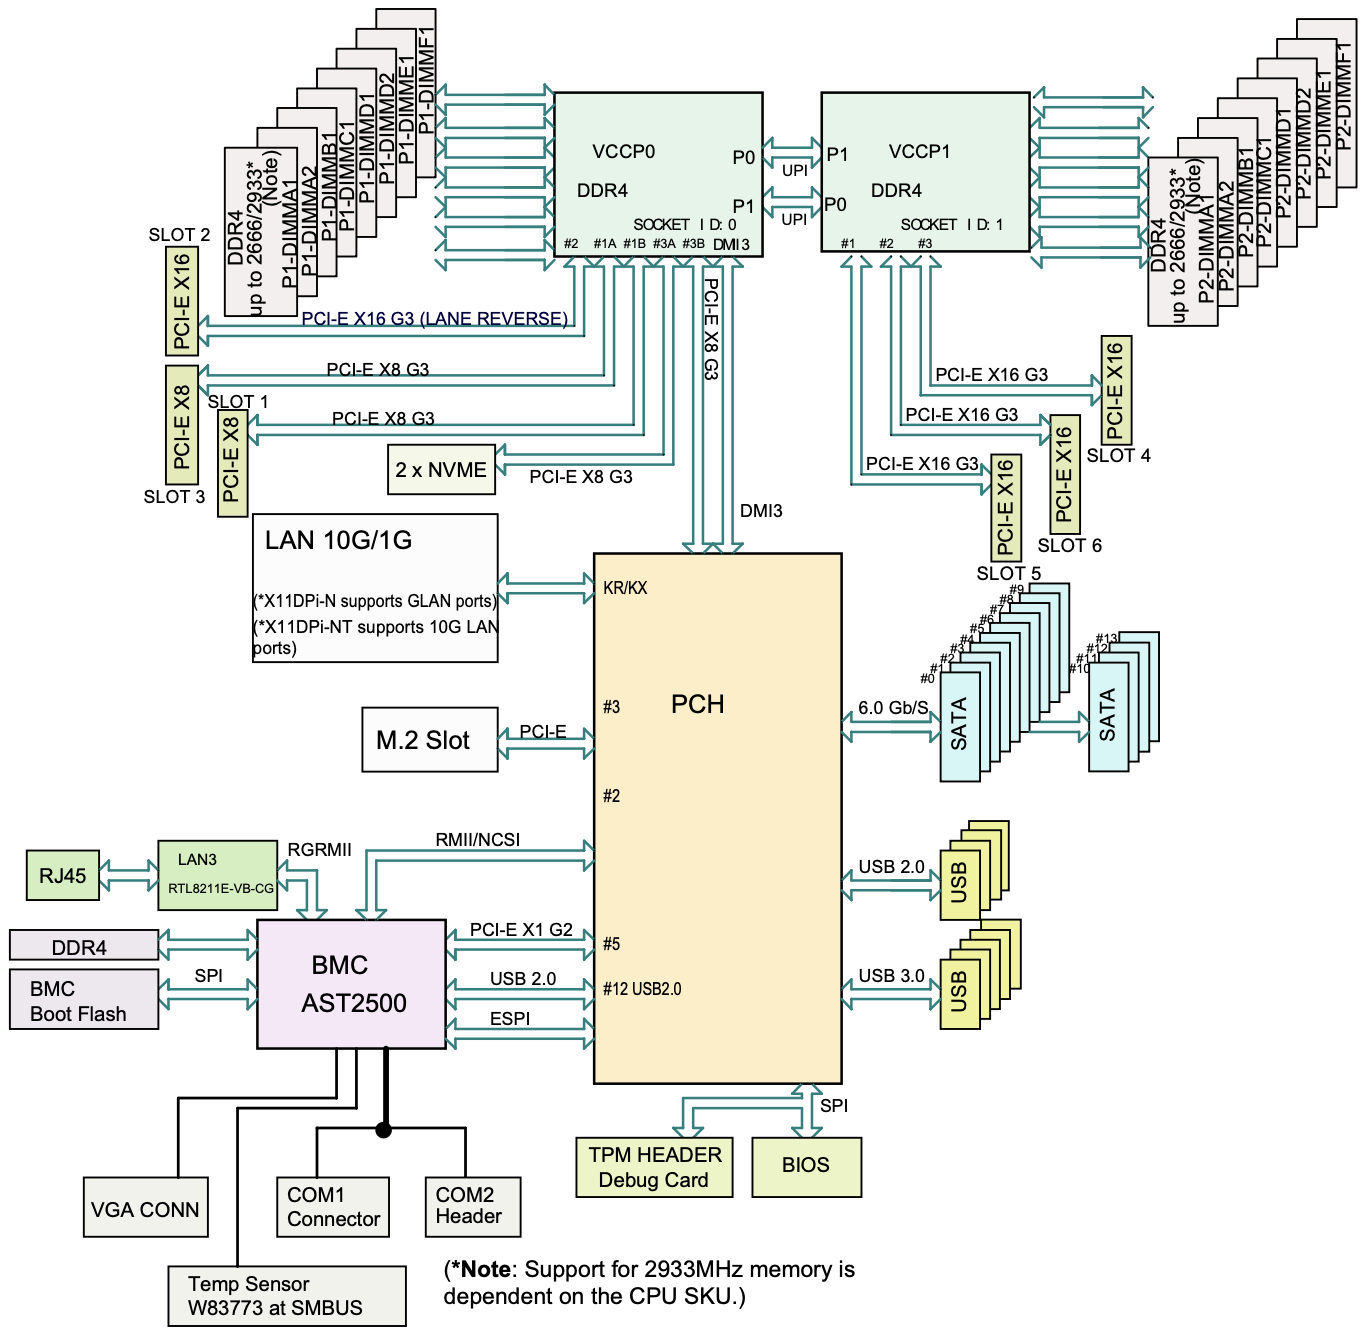
\includegraphics[width=1\linewidth]{figures/method/image1.png}
    \caption[Block Diagram of the Supermicro X11-DPi-N Mainboard]{Block Diagram of the Supermicro X11-DPi-N Mainboard. Source: \cite{setup05}.}
    \label{fig:BlockDiagrIHawk}
\end{figure}

The iHawk is a dual-socket system, as shown in the block diagram (Figure \ref{fig:BlockDiagrIHawk}). It utilizes a NUMA (Non-Uniform Memory Access) memory design, which means that memory performance varies at different points in the address space, depending on whether it is local memory or the memory of the other processor. Typically, access to local memory is significantly faster than to the memory of the other processor. A CPU with its local memory is referred to as a NUMA node \cite{setup06}.

To access the memory of the other NUMA node, an interconnect between the sockets is used. This can lead to potential problems such as:

\begin{itemize}
\item Increase in latency for memory access
\item Throughput bottleneck
\end{itemize}

The iHawk system utilizes two Intel Ultra Path Interconnect (UPI) links, as illustrated in Figure \ref{fig:BlockDiagrIHawk}.  Each link operates at a speed of 10.4 GT/s, providing a total full-duplex bandwidth of 41.6 GB/s \cite{setup08}. Accessing memory from the other NUMA node via the UPI increases latency by approximately 50\% \cite{setup06}, resulting in a memory latency of around 130 ns \cite{setup07} between the two sockets.

The block diagram shows that each PCI Express slot is connected to one CPU. Slots 0 to 3 are connected to CPU 0, while slots 4 to 6 are connected to CPU 1. It is important to note that the problems previously described for memory accesses also apply to accessing PCI Express devices on the other NUMA node, as they are also carried out via the UPI links.


\subsubsection{Network Hardware}

\paragraph{Ethernet Switch} \label{chap:EthernetSwitch}
The Ethernet switch used is a Cisco CBS350-8XT from the Cisco Business 350 series. It is a Layer 3 managed switch that supports 10 GbE. Its specifications are as follows \cite{setup09}:

\begin{itemize}
\item 8x RJ45 10 GbE Ports
\item 2x SPF+ (shared with RJ45 Port)
\item 160 GBit/s switching capacity
\item 6 MB packet buffer dynamically shared across all ports
\item Quality of Service (QoS) with 8 hardware queues
\item Support for jumbo frames with a maximum size of 9000 bytes
\end{itemize}

The Cisco CBS350-8XT is a Layer 3 switch that can forward packets based on both MAC and IP addresses, similar to a router.  However, for the purposes of the tests conducted in this thesis, this functionality was not required, so the switch was configured as a Layer 2 switch.

\paragraph{Network Interface Cards}

The tests only use PCIe Network Interface Cards (NIC) that are capable of 10 GbE. The main types of network interfaces used are Intel's X520-DA2, X540-T2, and X710-T2L. Network interfaces from Lenovo and Inspur are also considered. Table \ref{tab:NWHardware} provides a concise overview of the network interfaces used according to \cite{setupnw01, setupnw02, setupnw03, setupnw04}.

\begin{figure}[h]
    \centering
    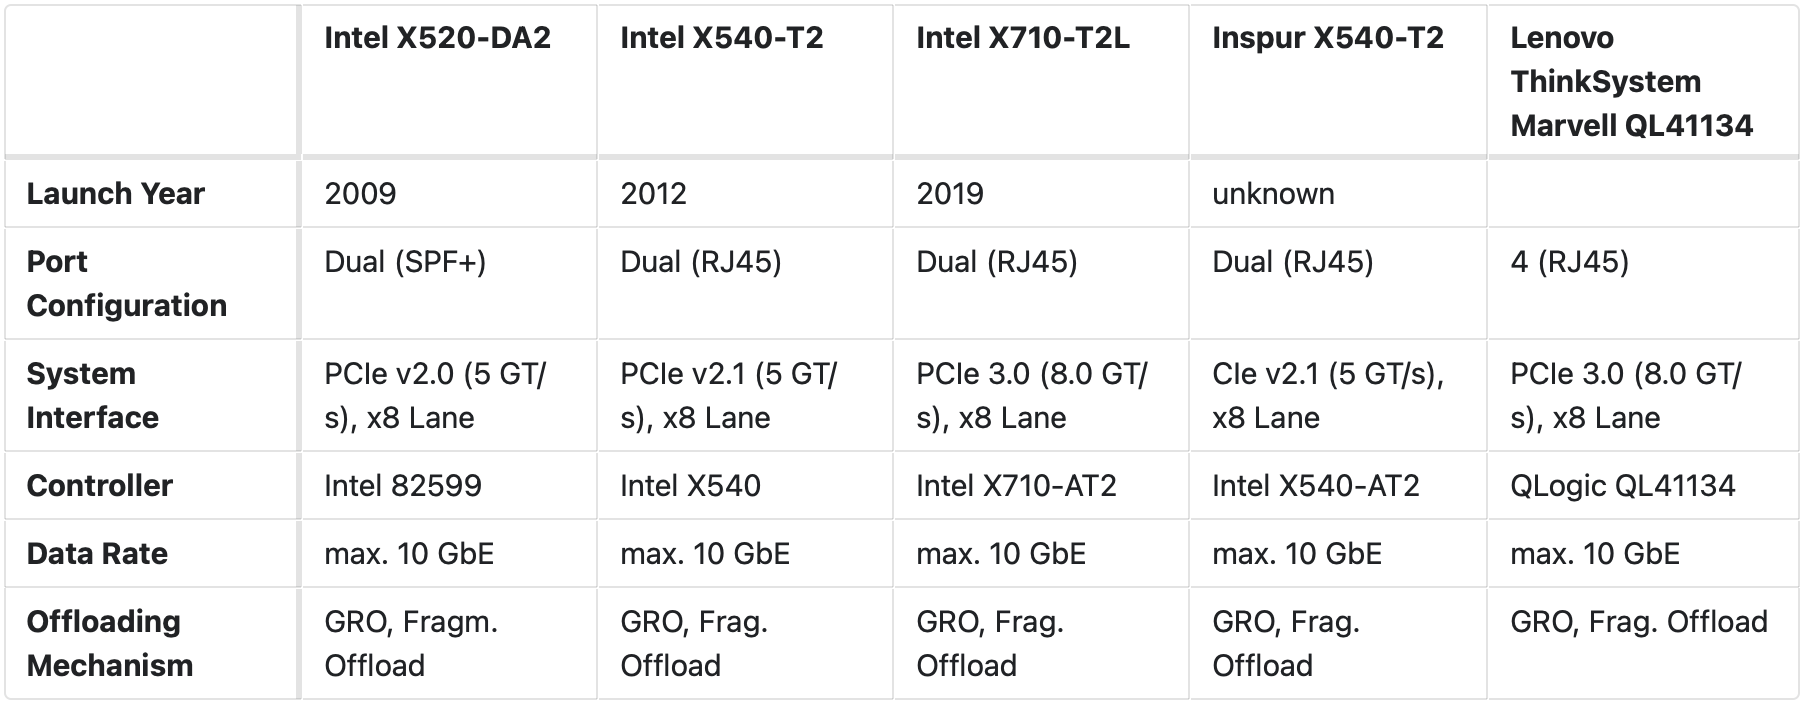
\includegraphics[width=1\linewidth]{figures/method/temp1.png}
    \caption{TODO - THIS SHOULD BE UPDATED TO A TABLE}
    \label{tab:NWHardware}
\end{figure}

The network interfaces were selected broadly to reduce dependence on specific interfaces or manufacturers. Additionally, network cards of varying ages and prices were considered to account for potential hardware limitations.

Chapter \ref{chap:Architectures} explains for each topology which network interfaces are used on which computer system. It should be noted that the Intel X710-T2L network interfaces are not compatible with computer systems of the 'Traffic PC' type.


\subparagraph{Comparison with Network Interfaces in the Test Support System}

In the distributed test system, for systems similar to the 'High Performance PCs' and the iHawk, a wide range of PCIe 10GbE network interfaces can be used. However, the CompactPCI Serial systems can only use network interfaces for which a corresponding peripheral module is available.

The Distributed Test System utilizes the SN5-TOMBACK peripheral module from EKF \cite{setupnw05}. This module uses the Intel 82599 controller, has two SPF+ ports and supports 10 GbE. It is therefore comparable to the Intel X520-DA2 network card in the test setup, which uses the same controller.

\paragraph{Cabling}
The cabling of the hardware used was carried out using Cat7 Ethernet patch cables with RJ45 plugs or with fiber optic cables and Intel SPF+ SR modules. Both cabling systems used are suitable for 10 GbE.

\subsection{Software Setup}
This chapter describes the software versions used and important configurations.

\subsubsection{Versions}
\paragraph{Operating System}
The operating system used on all computer systems is the real-time operating system RedHawk Linux 9.2 based on Ubuntu 22.04.3 LTS.

\begin{itemize}
\item \textbf{Operating system:} RedHawk 9.2 with Ubuntu 22.04.3 LTS user environment
\item \textbf{Linux kernel:} 6.1.19-rt8-RedHawk-9.2-trace
\end{itemize}

RedHawk Linux 9.2 is a real-time operating system developed by Concurrent, optimized for real-time determinism with precise and consistent response times and low latency \cite{swsetup01}. The manufacturer integrates open source patches and proprietary enhancements into the Linux kernel. The following list briefly describes some important features of the real-time optimized Linux kernel from the product brochure \cite{swsetup02}:

\begin{itemize}
\item \textbf{Standard Linux API}: Since RedHawk is based on a Linux kernel, it offers all standard Linux user level APIs such as POSIX. Therefore, applications created for other Linux distributions can also be executed on the operating system.
\item \textbf{Frequency-Based Scheduling}: RedHawk has a Frequency-Based Scheduler, which allows processes to be executed in a cyclical execution pattern driven from a real-time clock.
\item \textbf{Processor Schielding}: RedHawk enables the shielding of individual cores from timers, interrupts, or other Linux tasks, providing a deterministic execution environment.
\item \textbf{Multithreading and Preemption}: RedHawk allows multiple processes to execute simultaneously in the kernel while protecting critical data or code sections with semaphores or spinlocks. In the RedHawk kernel, processes can be preemptively interrupted to reallocate CPU control from a lower-priority to a higher-priority process, except during execution in critical kernel sections. To ensure deterministic responses, critical sections of the kernel have been optimized to reduce non-preemptable conditions and enabling high-priority processes to immediately respond to external events, even when the CPU is actively engaged.
\end{itemize}

RedHawk Linux was chosen for the test setup as it is also used in the Distributed Test System. It also offers low latency, which should have a positive impact on the performance characteristics.

\paragraph{Drivers of the Network Interface Cards}

The drivers supplied with the kernel are used for the network cards. Table \ref{tab:drivernic} lists the drivers used for the network cards.

\begin{table}[h]
\centering
\begin{tabular}{ll}
	\toprule
	Driver & Network Interface Card\\
	\midrule
	i40e & Intel X710-T2L\\
	ixgbe & Intel X520-DA2, Intel X540-T2, Inspur X540-T2 \\
	qede & Lenovo ThinkSystem Marvell QL41134\\
	\bottomrule
\end{tabular}
\caption{Overview of the Drivers of and the associated Network Interface Cards.}
\label{tab:drivernic}
\end{table}

\subsubsection{Configurations}
This chapter describes the general configurations that were used for all tests.

\paragraph{Activation of Jumbo Frames}

The tests used jumbo frames with a maximum size of 9000 bytes. Jumbo frames must be supported by all network nodes to avoid packet loss \cite{swsetup04}. Since the network in the test setup and in the distributed test system is completely under user control, no problems are expected in this regard. \\

\begin{lstlisting}[language=Bash, caption=Configuration of Jumbo Frames for the ethX Interface., label=lst:jumbocongif]
ifconfig ethX mtu 9000
\end{lstlisting}

Listing \ref{lst:jumbocongif} shows the configuration of jumbo frames with a maximum size of 9000 bytes for the \textit{ethX} interface.


\paragraph{Real-time Process} \label{chap:RTProcess}
The tests, specifically the test program described in the following section \ref{chap:TestSuite}, were executed as a real-time process with the highest priority. This was done in order to obtain realistic test conditions, as the communication layer is also executed as a real-time process in the distributed Test System. \\

\begin{lstlisting}[language=Bash, caption=Modification of the real-time Attributes of a Process., label=lst:rtprocess]
chrt -f -p 99 [PID]
\end{lstlisting}

Listing \ref{lst:rtprocess} contains the command used to modify the real-time attributes of a process with a specific PID (Process ID). The same command was also applied to the test program. According to \cite{swsetup05}, the real-time attributes were modified as follows:

\begin{itemize}
\item Change of the \textbf{scheduling policy} to \texttt{SCHED\_FIFO}. This is a first in/first out realtime scheduling policy through which the processes have a higher priority than all normal processes and can interrupt them at any time \cite{swsetup06}.
\item Change of the \textbf{scheduling priority} to 99. \texttt{SCHED\_FIFO} uses a fixed priority with values ranging from 1 to 99, with 99 as the highest priority \cite{swsetup06}.
\end{itemize}



\section{Network Topologies} \label{chap:Architectures}
For the tests with the described setup, two different topologies were utilized for the local Ethernet network and the arrangement of the computer systems. Both topologies are star-shaped, consisting of bidirectional point-to-point links that connect two systems. Each link can be used independently in both directions \cite{Tanenbaum2010}.


\begin{figure}[h]
    \centering
    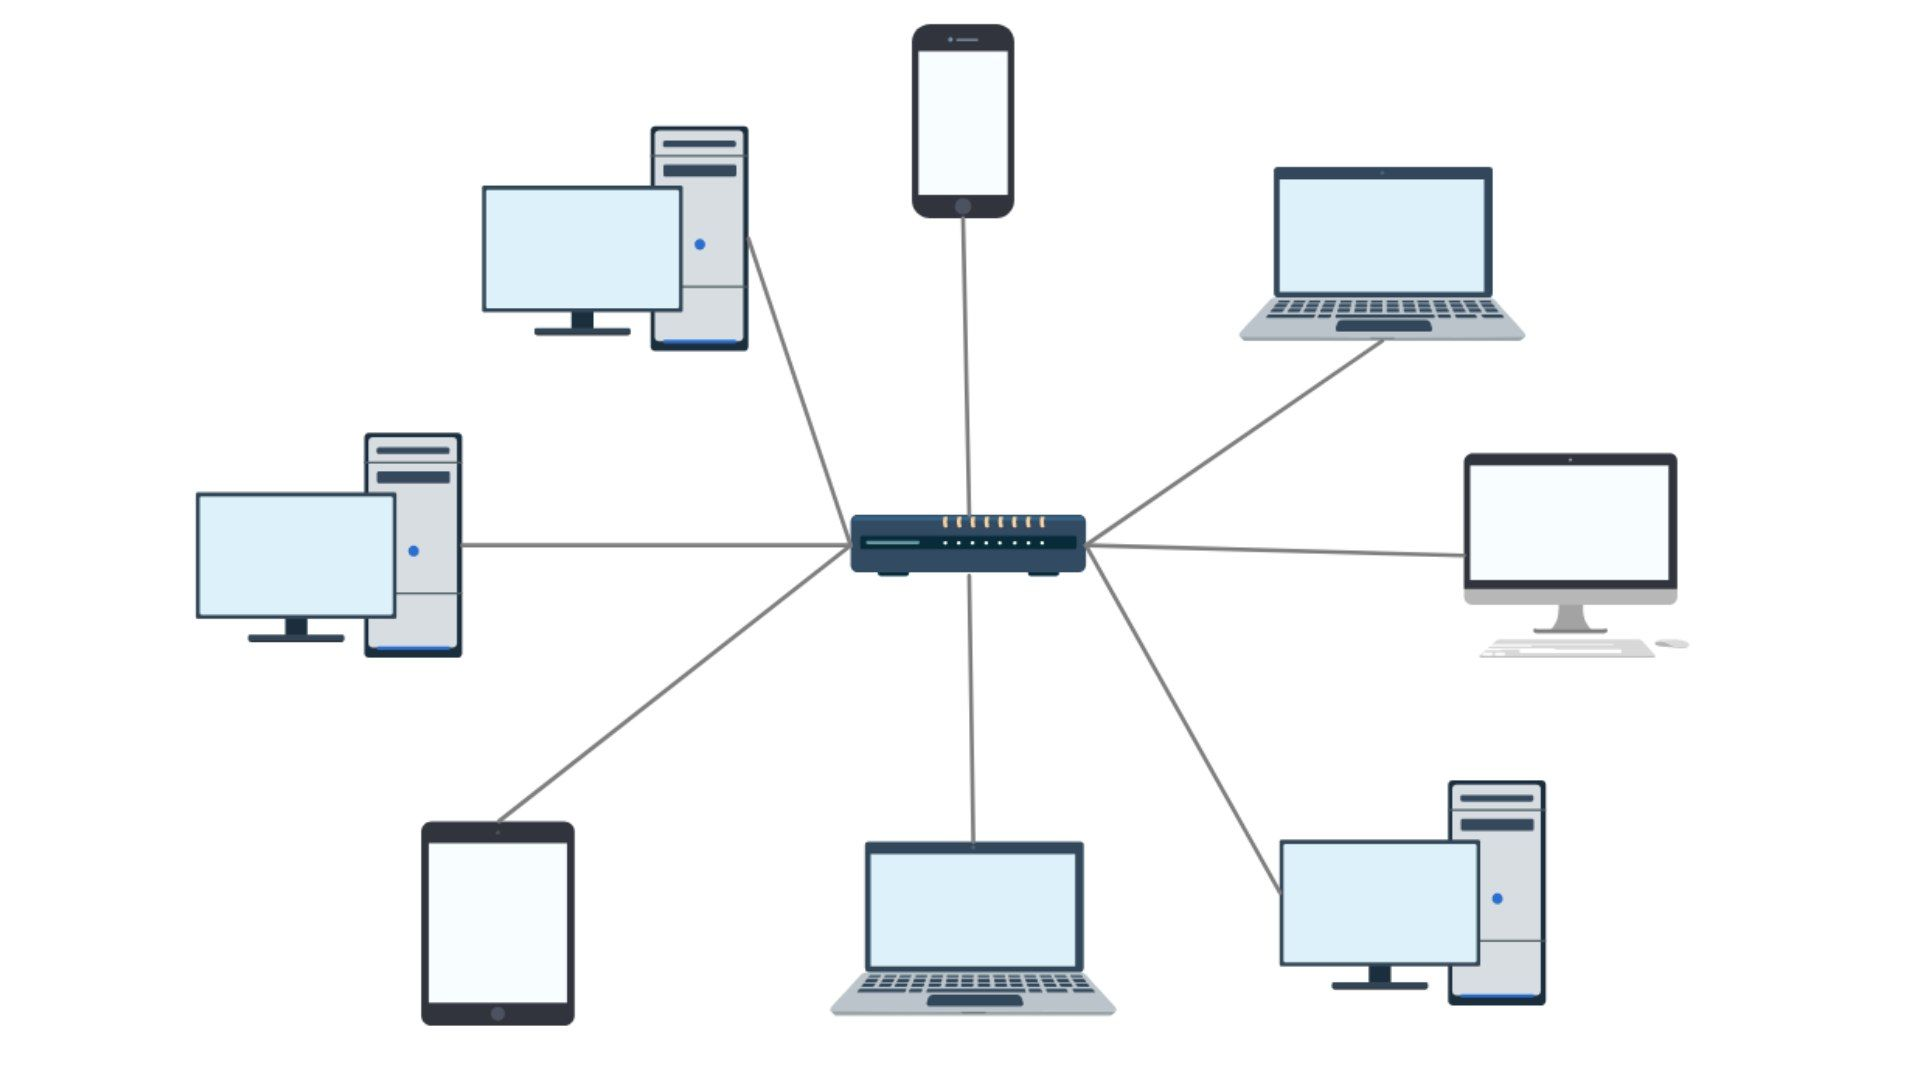
\includegraphics[width=0.6\linewidth]{figures/method/topo1.png}
    \caption[Structure of a generic Star Topology]{Structure of a generic Star Topology. Source: \cite{topo01}.}
    \label{fig:startopoGeneral}
\end{figure}

In a star topology, each node connects to a central instance, typically a hub or a switch. A generic star topology is shown in Figure \ref{fig:startopoGeneral}. The advantages of the star topology are simple installation and high fault tolerance, as the network remains functional if a node fails. However, if the central instance fails, the network becomes non-functional. Additionally, more cabling is necessary.

Both topologies used are described in detail below. Any modifications made for specific test campaigns are indicated in the corresponding places in the thesis. This includes, for example, changes to the network interfaces used.

\subsection{Star Topology with a Switch in the Center}

\begin{figure}[h]
    \centering
    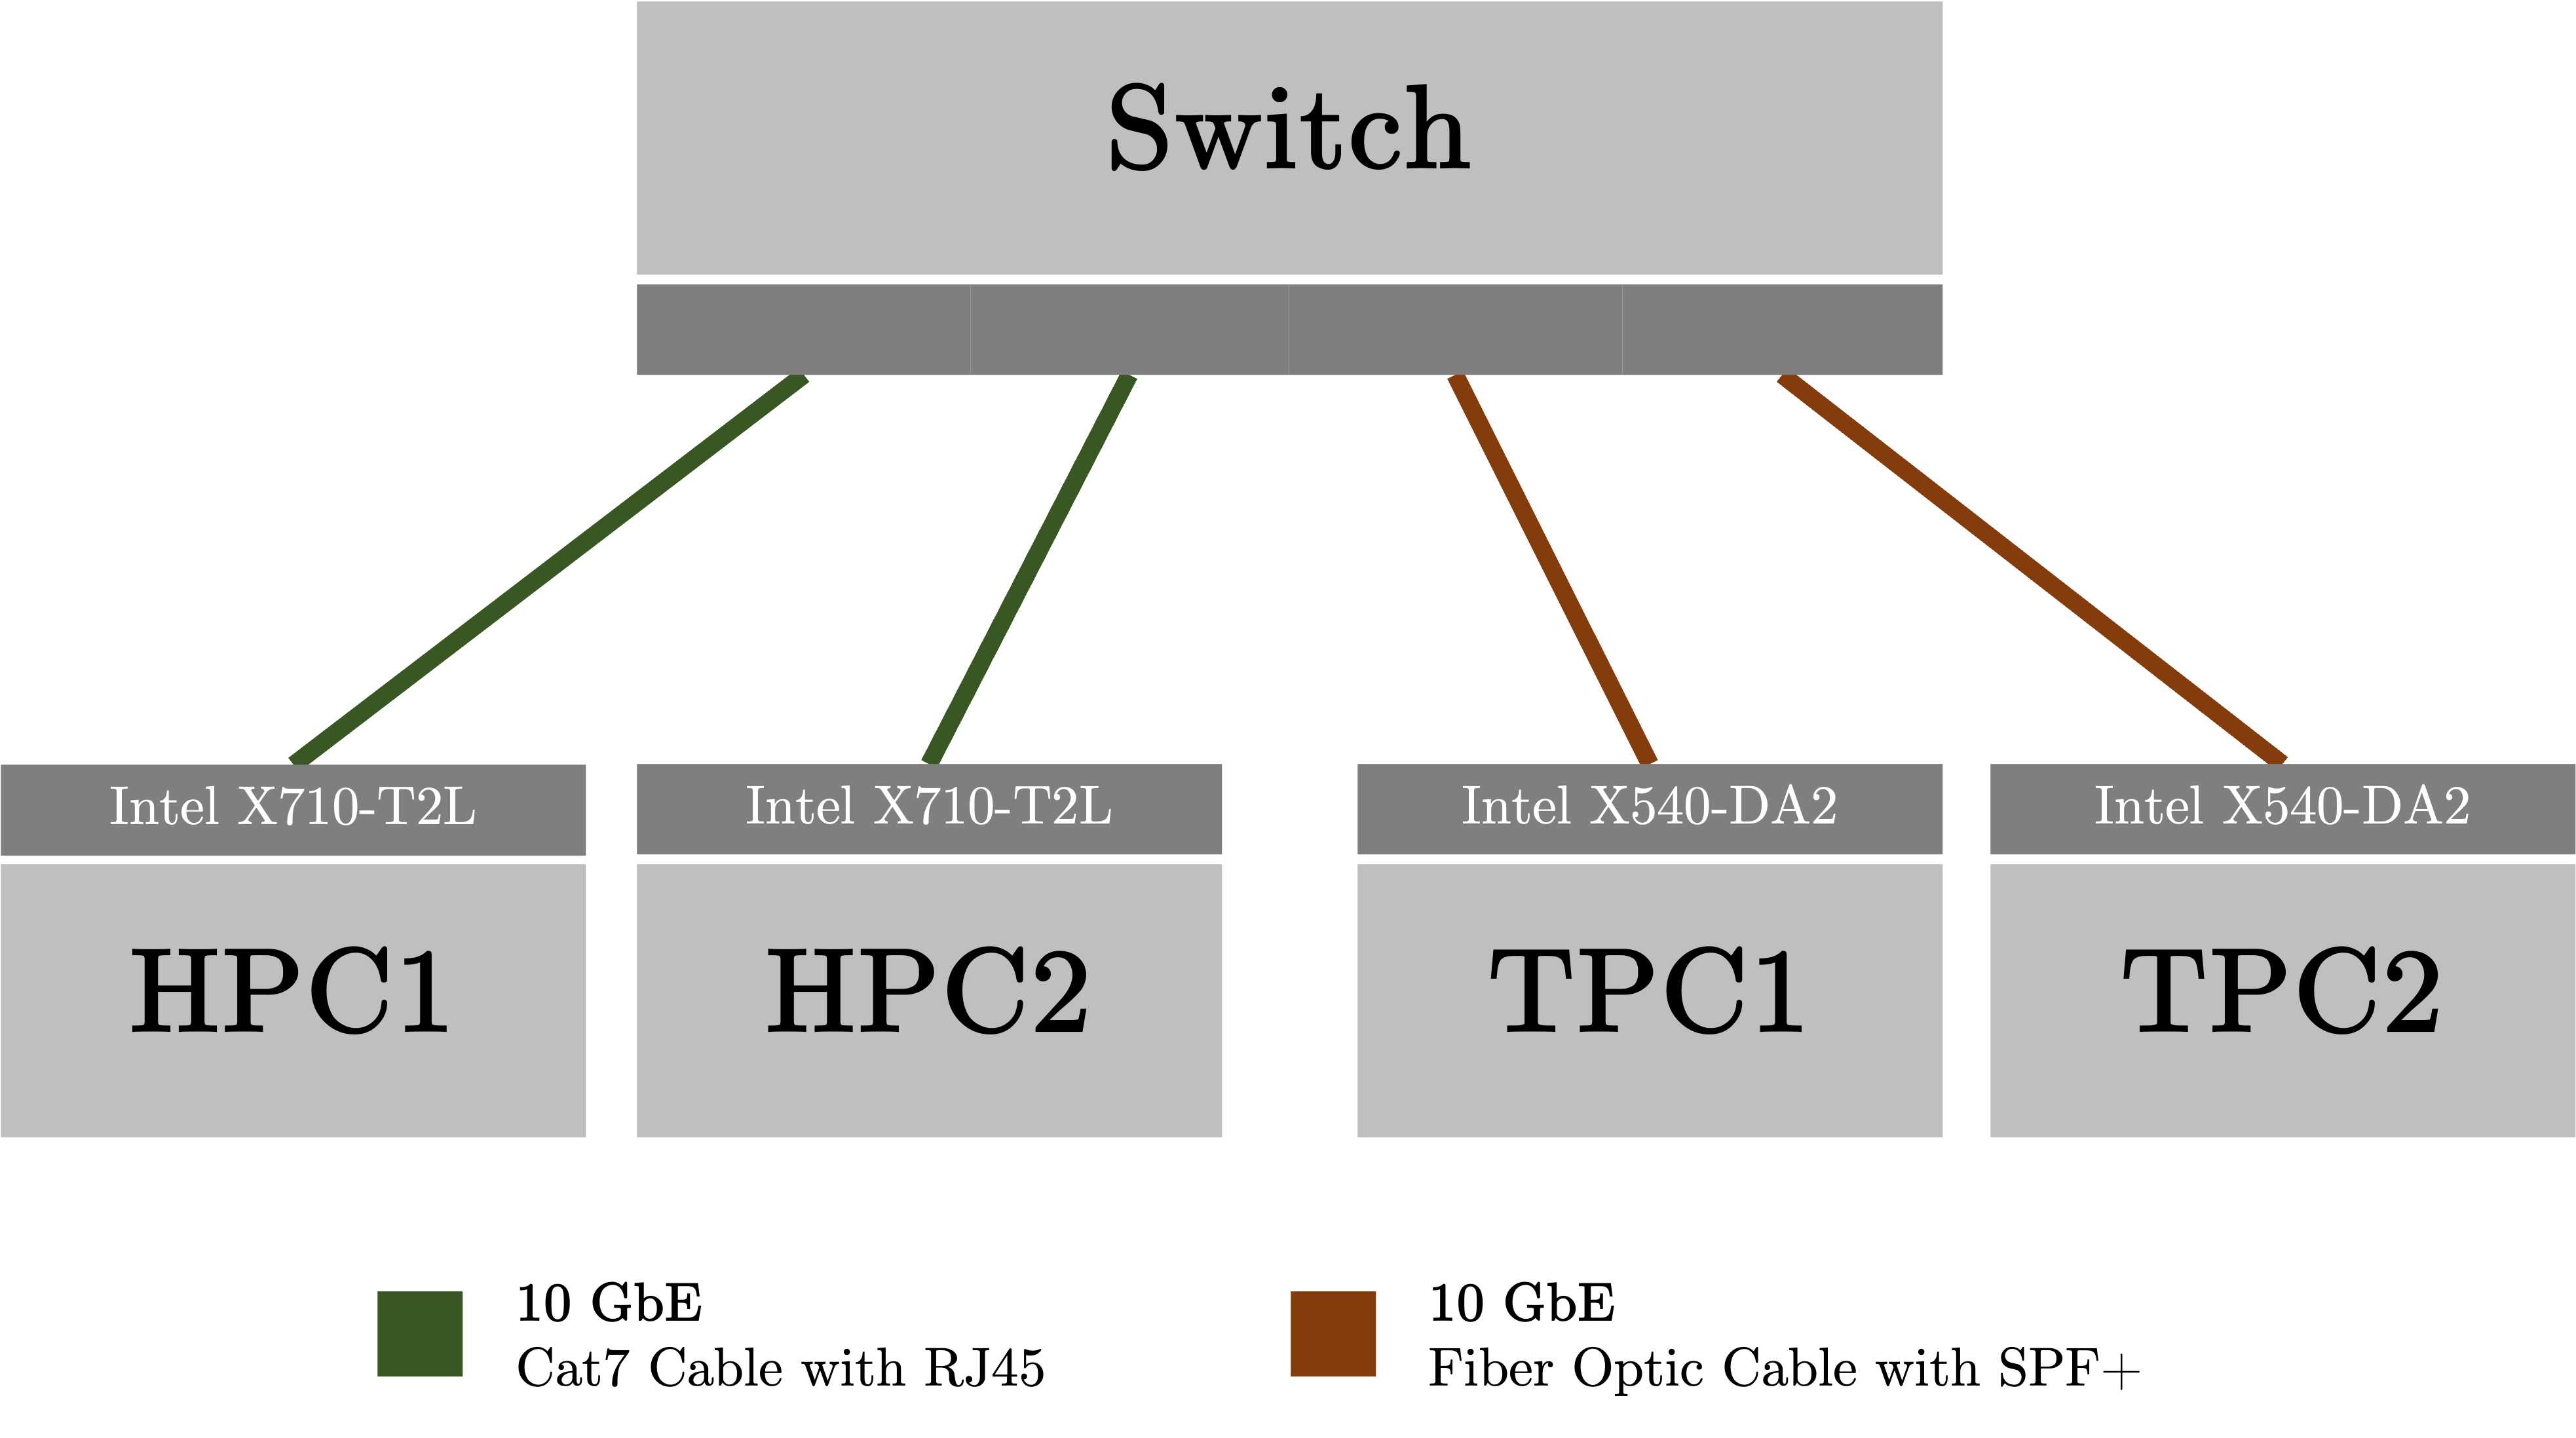
\includegraphics[width=1\linewidth]{figures/method/topo2.png}
    \caption[Visualization of the Star Topology with a Switch in the Center]{Visualization of the Star Topology with a Switch in the Center.}
    \label{fig:startopoSwitch}
\end{figure}

The first topology used is a star topology with a switch in the center, as shown in Figure \ref{fig:startopoSwitch}.

In this architecture, the Cisco CBS350-8XT switch, presented in \ref{chap:EthernetSwitch}, is located in the center of the star. All other participants, including two computer systems of type HPC and the computer systems of type TPC, are connected to this switch.

The HPC1 and HPC2 systems are both equipped with the Intel X710-T2L network card and are each connected to the switch with a bidirectional link using Cat7 copper cables. The TPC1 and TPC2 systems were equipped with the Intel X540-DA2 network card, which has SPF+ ports. They were connected to the switch via fiber optic cables using Intel SPF+ SR transceivers.

\subsection{Star Topology with the iHawk in the Center}

\begin{figure}[h!]
    \centering
    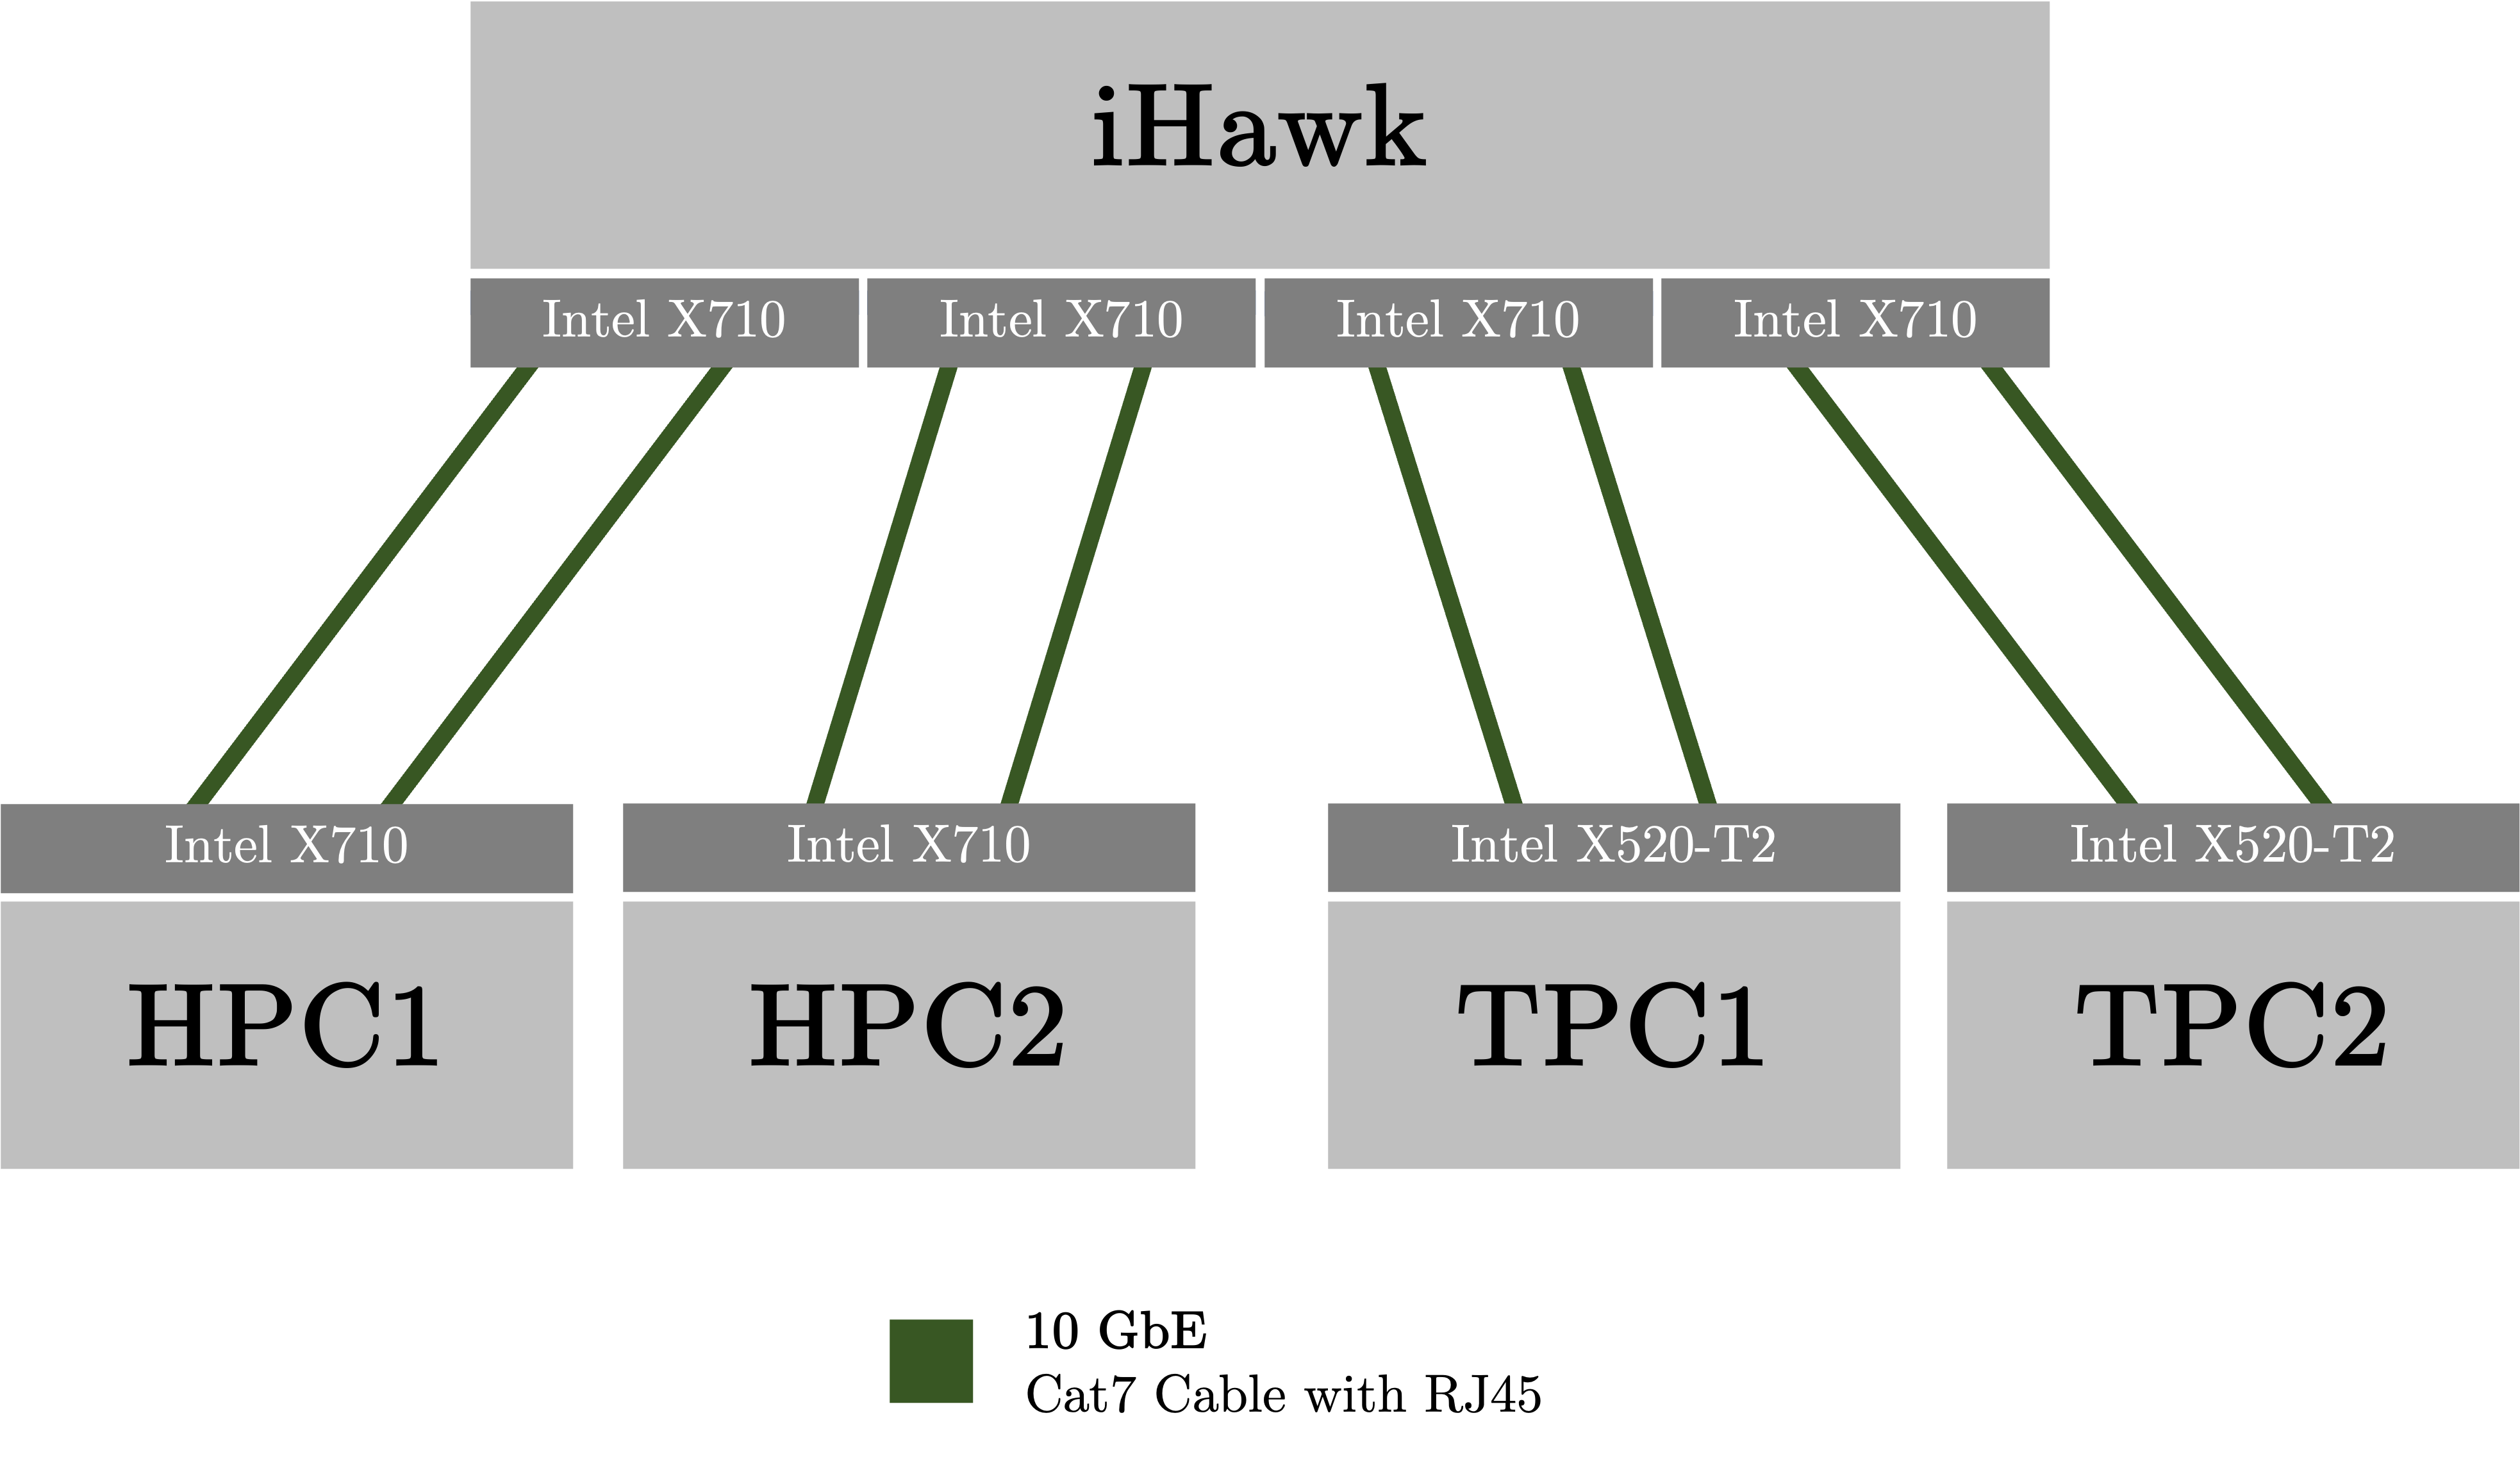
\includegraphics[width=1\linewidth]{figures/method/topo3.png}
    \caption[Visualization of the Star Topology with the iHawk in the Center]{Visualization of the Star Topology with the iHawk in the Center.}
    \label{fig:startopoIHawk}
\end{figure}

As the first topology presented proved to be unsuitable in the course of the tests carried out, a new topology as shown in Figure \ref{fig:startopoIHawk} was developed.

This new topology features an iHawk computer system at the center of the star, equipped with four Intel X710-T2L network interfaces. The HPC computer systems in this topology also have Intel X710-T2L network interfaces, while the TPC systems use Intel X520-T2 network interfaces. Each node is connected to the iHawk in the center via two bidirectional 10 GbE links.


\section{Introduction of the Test Program} \label{chap:TestSuite}
A dedicated test program, called TestSuite, was created to carry out the tests with the setup described above. The decision to create an own test program was based on the following considerations, which were not fully covered by existing network performance test programs such as iPerf \cite{testsuite01}:

\begin{itemize}
\item \textbf{Execution of tests with UDP protocol}: TestSuite focuses exclusively on tests with the UDP protocol and offers various setting options with regard to the generated and measured UDP communication. In addition to UDP sockets, RAW and PACKET sockets are also supported.
\item \textbf{Results management}: TestSuite saves all relevant results of a test run in XML files, which facilitates subsequent evaluation.
\item \textbf{Focus on relevant aspects of the test}: The TestSuite places particular emphasis on testing packet loss and latency. This is reflected in various functionalities that stand out from existing test programs:

	\begin{itemize}
      \item Recording of losses with intermediate results throughout the test
      \item Recording of additional metrics for more precise investigation of packet losses
      \item Recording of send and receive timestamps for each packet
    \end{itemize}

\item \textbf{Automation of tests}: Due to the large number of tests that were expected in advance, the tests can be automated. This allows a more optimized utilization of the test setup to be achieved. Furthermore, required environmental conditions in the system, such as an additional system load, can be generated automatically.
\end{itemize}

Disadvantages of creating a custom test program is the additional time required for development and the presence of possible errors that could falsify the results. As the advantages listed above outweighed the disadvantages, the decision was made to develop the TestSuite.

This section first describes the software design of TestSuite. This is followed by a more detailed description of the communication generated and measured by TestSuite. Then, the interpretation and evaluation of the data generated during a test run will be considered and the relevant results recorded by TestSuite will be presented. The complete source code of the TestSuite can be found in the appendix.


\subsection{Software Design}
The TestSuite was developed using the C++ programming language in the C++20 version. The concept of object-oriented programming has been used. The Qt Creator IDE was used for programming. In the following, the concept of the TestSuite is explained before the architecture of the software is explained.

\subsubsection{Concept}

\begin{figure}[h!]
    \centering
    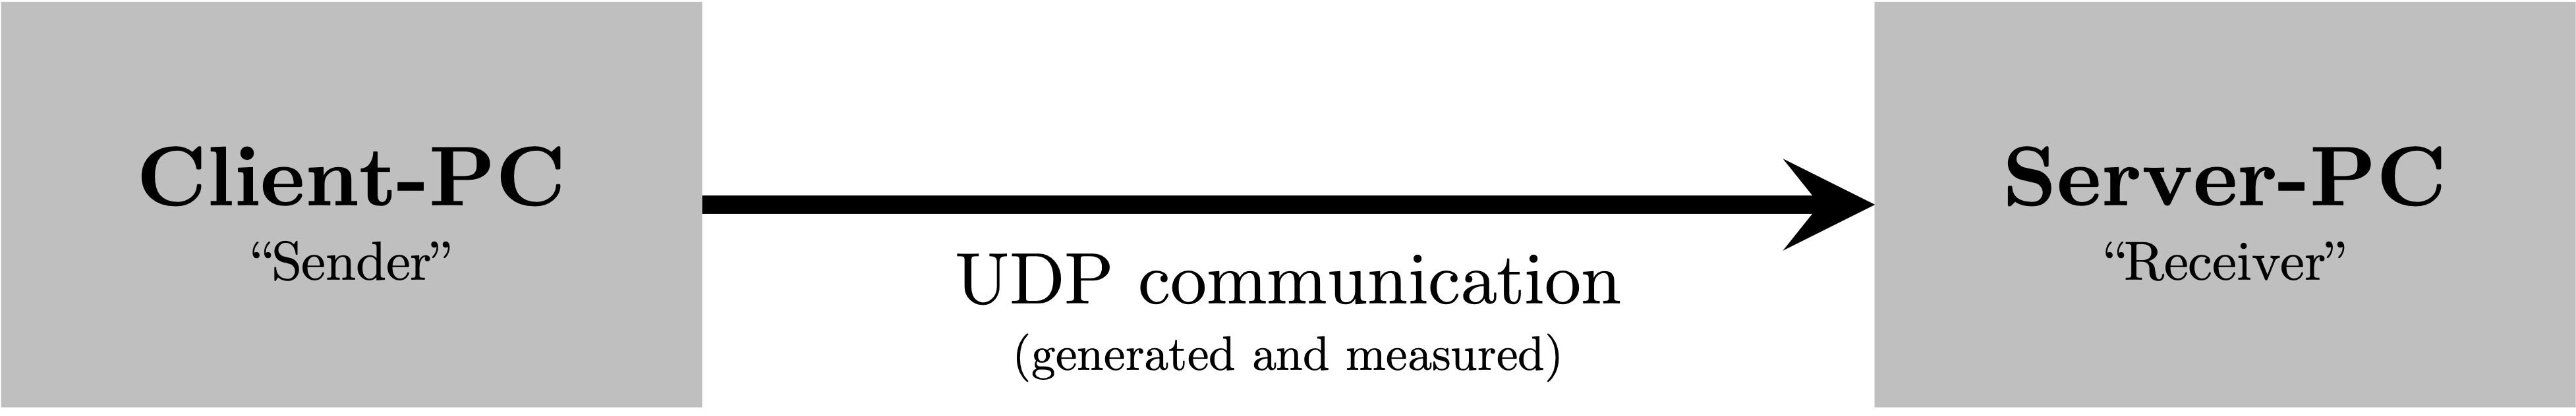
\includegraphics[width=1\linewidth]{figures/method/swdesign1.png}
    \caption[Illustration of the TestSuite Concept]{Illustration of the TestSuite Concept.}
    \label{fig:tsconcept}
\end{figure}

The TestSuite is designed for reliability and performance testing with the topologies presented in \ref{chap:Architectures}. The basic concept of the TestSuite is shown in Figure \ref{fig:tsconcept}. TestSuite always generates and measures a UDP communication between a sender, also called a client, and a receiver, also called a server. The focus of TestSuite is on tests performed between two participants in a local network.

TestSuite is able to generate a UDP communication with a pre-defined payload and bandwidth and record associated metrics such as the number of lost packets or the latency between sending and receiving. The generated communication is a one-way communication, i.e. the server does not respond to messages from the client. One execution of TestSuite can generate and measure a maximum of one communication. If more than one communication is to be analyzed in a system, TestSuite can be executed multiple times.

\subsubsection{Architecture}

\begin{sidewaysfigure}
    \centering
    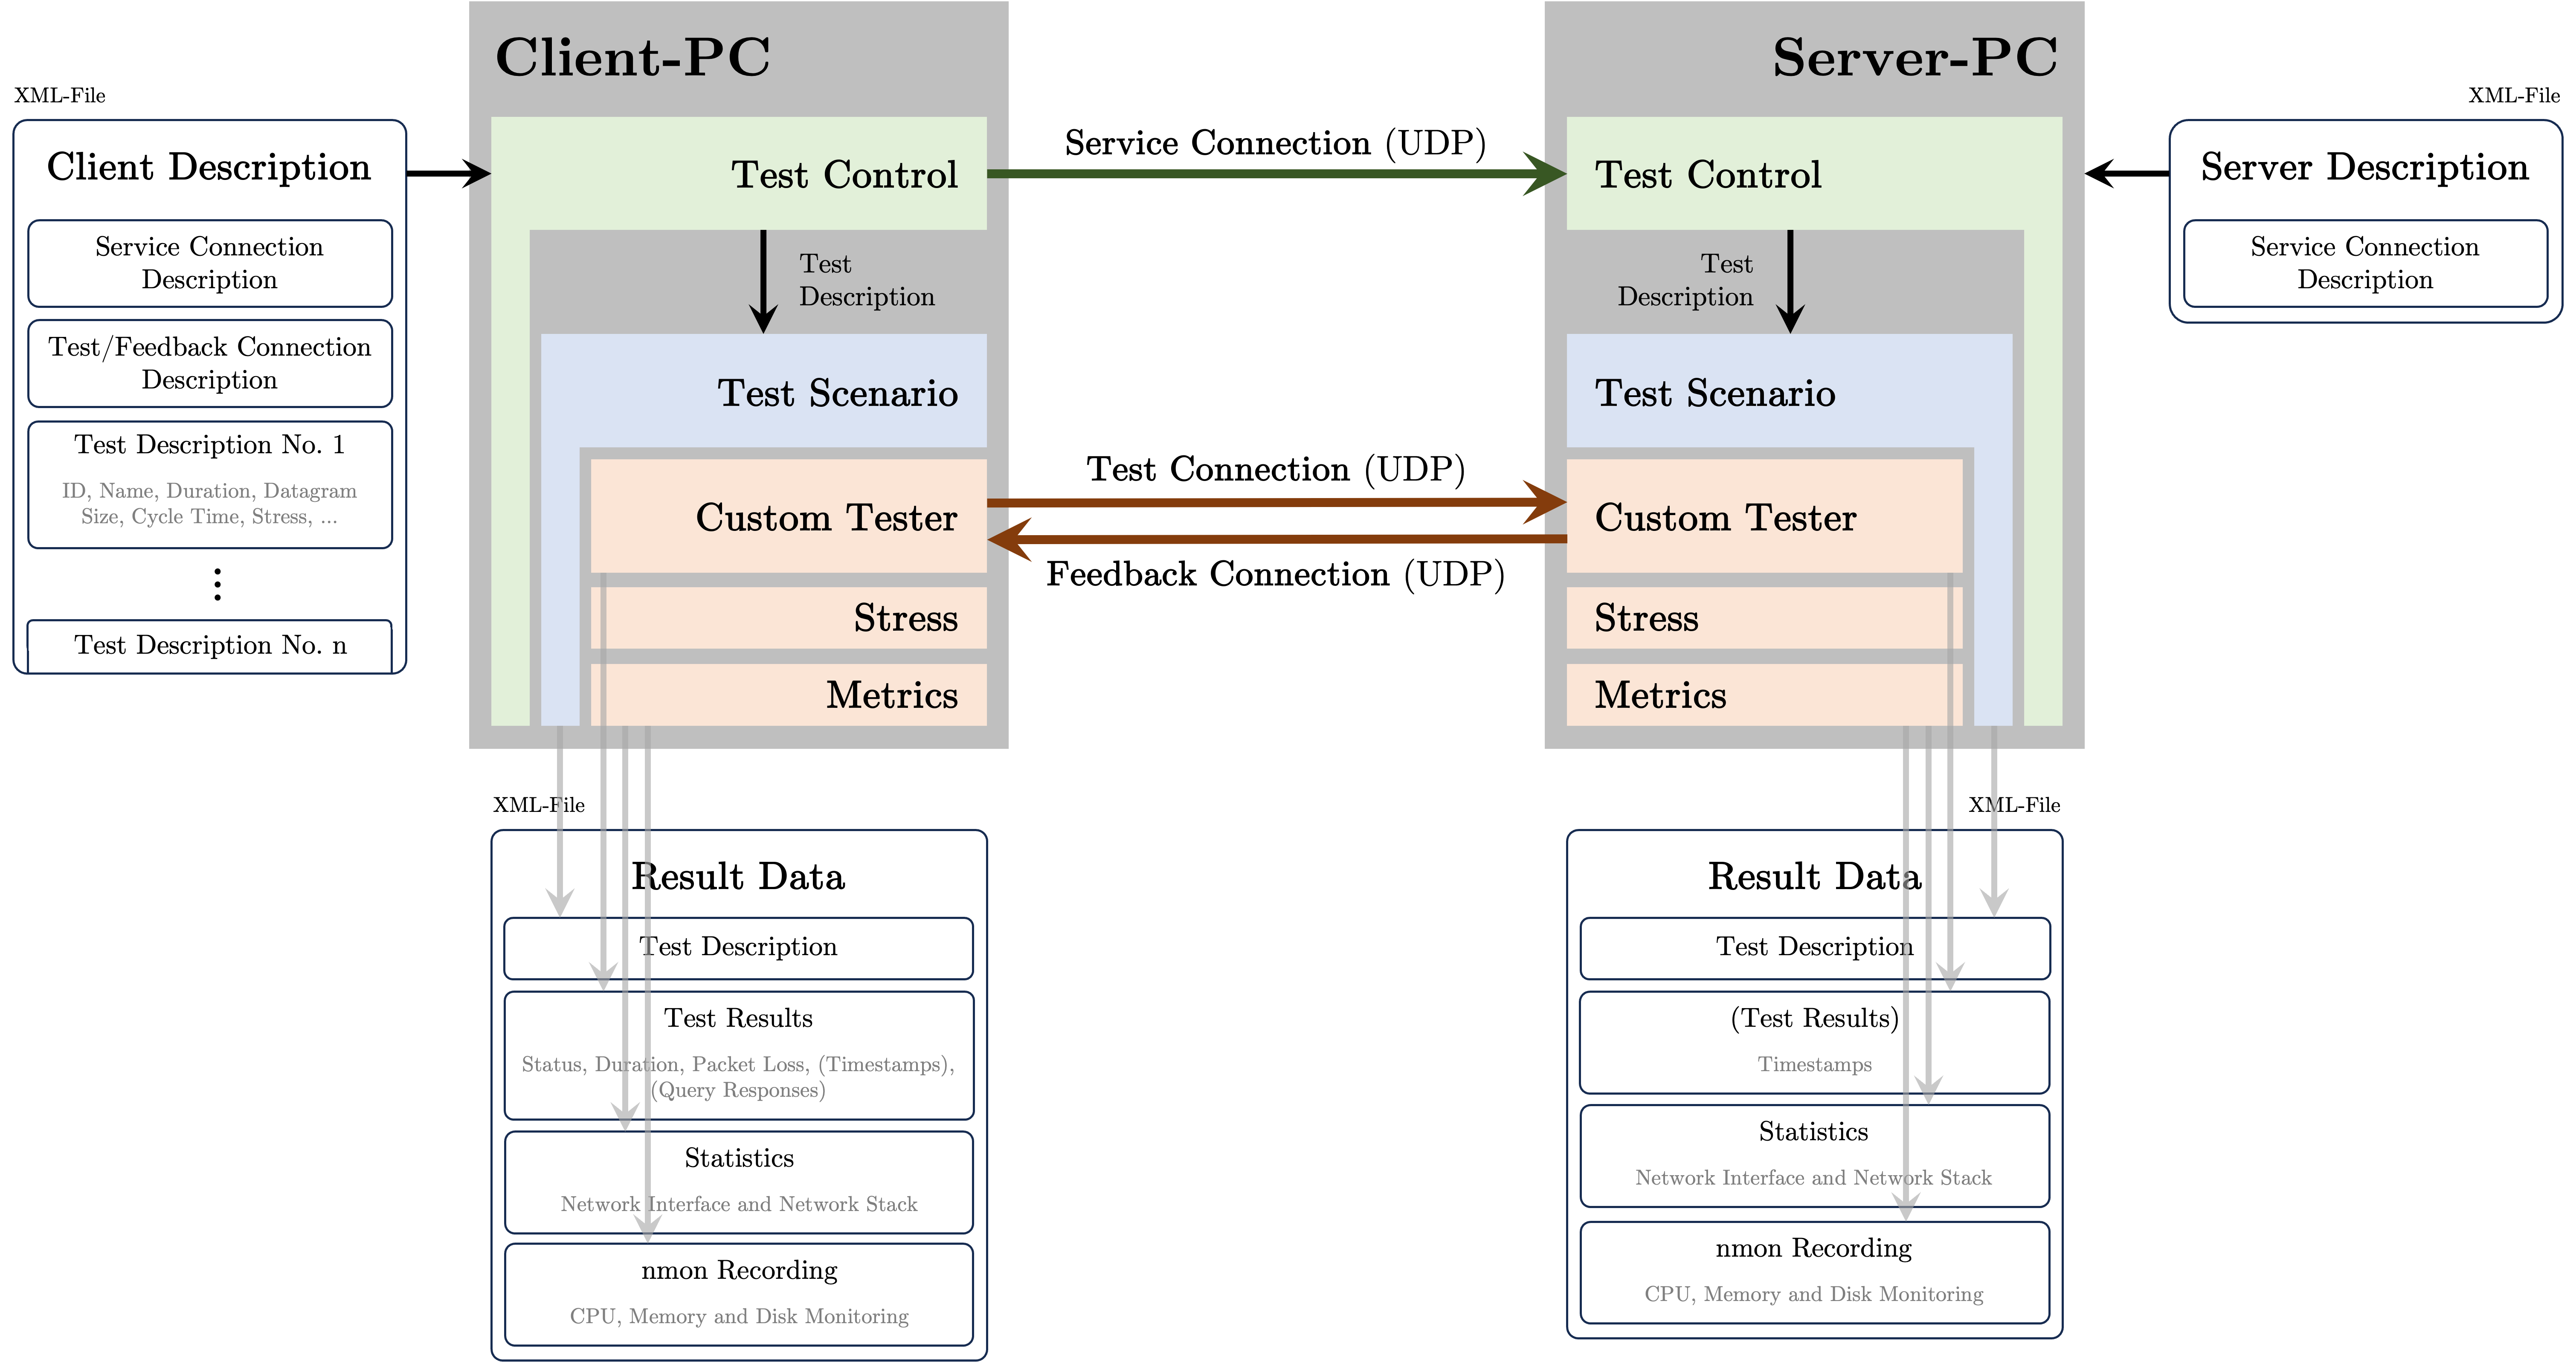
\includegraphics[width=1\linewidth]{figures/method/swdesign2.png}
    \caption[Architecture of the TestSuite with the relevant Classes, Data and Connections between the Systems]{Architecture of the TestSuite with the relevant Classes, Data and Connections between the Systems.}
    \label{fig:tsarch}
\end{sidewaysfigure}

Figure \ref{fig:tsarch} shows the architecture of TestSuite in a simplified form. The central elements are the systems on which TestSuite is executed. These are the client PC and the server PC. The client PC is also responsible for controlling the execution of the tests.

The input and output data is also shown. The diagram also shows the five central classes of the application and their hierarchy, as well as the various communication channels between the client PC and the server PC. The following sections describe these components in more detail.

\paragraph{Communication Channels}
Communication between the client PC and the server PC takes place via three separate communication channels, all using the UDP protocol.

The 'Service Connection' is used to send configuration data to the server. This includes the description of the tests to be performed and the starting and stopping of a test execution. Furthermore, the configurations of the other communication channels, the 'Test Connection' and the 'Feedback Connection', are sent to the server.

The UDP protocol is used for the 'Service Connection'. This is due to the fact that TestSuite focuses on tests between two participants in a local network. However, UDP does not guarantee that the packets sent will reach their destination. Therefore, if TestSuite is to be used for tests over external networks in the future, a protocol should be used that guarantees the reliability of its transmission.

The 'Test Connection' is the communication channel to be tested. A UDP communication is generated and measured according to certain parameters. This channel exists from the client to the server.

The 'Feedback Connection' allows the server to send messages to the client during the current test run. This is also a UDP connection. The server sends the requested data only when requested by the client.

\paragraph{Input and Output Data}
All data required or created by TestSuite is written in Extensible Markup Language (XML). XML is a markup language for storing structured data in text form \cite{tsd01}. Because XML allows hierarchical storage of data and is human readable, it was used in TestSuite.

The pugixml library was used to read, process and create the XML files in TestSuite. pugixml is a C++ library that allows easy and efficient processing of XML files. More information about pugixml can be found in its documentation \cite{tsd02}.

In the following, the input data of the TestSuite, 'Client Description' and 'Server Description', as well as the output data will be examined in more detail.

\subparagraph{Input Data}
The TestSuite contains all inputs and configurations in the form of a 'Client Description' or 'Server Description'. Both have a similar structure, but the Client Description is more comprehensive because the client is responsible for controlling the tests.

The first element present in both input files is a description of the 'Service Connection'. This is used to exchange test management data between the systems. The description includes the server's IP address and port.

Next, the 'Client Description' contains the configuration of the 'Test Connection' and the 'Feedback Connection'. This includes the IP addresses and port of both channels. In addition, the "Test Connection" description includes the names of the network interfaces used in the client and server, which are required to retrieve statistics. This communication channel also provides the option of using a RAW socket or a PACKET socket in addition to a UDP socket.

The 'Client Description' also contains a description of the tests to be performed, the so-called 'Test Description'. The Client Description can contain any number of Test Descriptions, which are executed in sequence.

The 'Test Description' is a central element of the TestSuite. It contains the complete description of a test execution and must be available in both the client and the server in order to run a test. The 'Test Description' includes:
\begin{itemize}
	\item \textbf{ID} and \textbf{name} of the test
	\item \textbf{Path} where the test results are stored
	\item \textbf{Duration} of the test
	\item Description of the communication to be generated with \textbf{datagram size} and \textbf{cycle time}
	\item Description of \textbf{stressors} for generating additional system load
	\item Configurations for \textbf{latency measurement} or the use of \textbf{query requests}
\end{itemize}

The data presented here is explained in more detail in \ref{chap:targetcom} This includes the configurations for generating communication, the generation of additional system load, latency measurement and query requests.

\subparagraph{Output Data}

Both the Client PC and the Server PC store their output data, called 'Result Data', in the form of XML files. The result data is re-generated for each test.

The first element of the 'Result Data' is the 'Test Description' of the test performed. This makes it easier to associate the output data with a specific test scenario and to analyze the results.

The output data also includes the test results. These vary depending on the test configuration, but typically include the following elements:
\begin{itemize}
	\item \textbf{Status} of the test execution (success or error)
	\item \textbf{Duration} of the test
	\item Number of packets \textbf{sent} and \textbf{received}, with intermediate results from the \textbf{query requests} if applicable
	\item \textbf{Timestamp} for the sending or receipt of each packet
\end{itemize}

The test results in the 'Result Data' for the server are less extensive. They usually only contain the timestamp for the arrival of each packet. The test results and their evaluation are discussed in more detail in Section \ref{chap:evaluationTS}.

The output data also contains statistics of the network interface or network stack in the respective system. These are recorded before the start and after the end of a test. The statistics are stored:
\begin{itemize}
	\item \textbf{Standard Interface Statistic} of used network interface: \\
	These statistics include the number of bytes and packets sent and received by the interface. They also include a counter for the number of packets dropped by the interface \cite{tsd03}.
	\item \textbf{Network Stack Statistic}: \\
	These statistics contain information about the protocol layer of the system. The information about UDP and IP is stored in the output data. This includes the number of packets sent and received by each protocol layer, as well as counters for dropped packets. The information about receive errors, such as insufficient buffer space, is particularly relevant for testing.
\end{itemize}

The output data also includes logs from the nmon tool. This is described in more detail in Section 2.3.X. The data includes minute-by-minute records of the system's CPU usage, memory usage, network interface data, and disk usage information.
% TODO

\paragraph{Classes}
TestSuite has 5 central classes, the functionality of which is briefly explained below.

\subparagraph{Test Control}
The 'Test Control' class is responsible for controlling and automating the execution of the test campaign. For this purpose, the class processes the input data of the TestSuite, the 'Client Description' or the 'Server Description'.

An important task is to control the execution of the tests. This is done by the 'Test Control' on the client PC. The tests contained in the Client Description are executed sequentially by creating an instance of the Test Scenario class for each test.

In addition, 'Test Control' in the client sends commands to start and stop a test and the 'Test Description' of the current test to the server via the 'Service Connection'. The server is then able to execute the test accordingly.

\subparagraph{Test Scenario}
The 'Test Scenario' class handles the overall management of a single test. To create an instance of the class, the 'Test Description' of that test is required as a parameter.

The class will then create instances of the necessary components for that test according to the specifications in the 'Test Description'. This includes:
\begin{itemize}
	\item Class 'Custom Tester'
	\item Class 'Stress'
	\item Class 'Metrics'
\end{itemize}

\subparagraph{Custom Tester} \label{chap:customtester}
The "Custom Tester" class is responsible for generating and measuring the UDP communication and processing the test results. The generation and measurement of target communication as well as the associated configuration parameters and technical details are described in \ref{chap:targetcom}.

The data measured during a test is then processed and saved as an XML file. "Custom Tester" saves the "Test Results" section of the "Results Data" output data structure.

\subparagraph{Stress}
The 'Stress' class is responsible for controlling the generation of additional system load during testing. This includes areas such as CPU load, I/O load, or network load.

The two programs 'stress-ng' and 'iPerf2' are used to generate these loads. These are described in more detail in Section \ref{chap:loadgeneration}. The 'Stress' class of TestSuite controls these external programs, including starting, stopping, and configuring them.

The additional system load can be executed during a test on the client PC or the server PC, or on both systems simultaneously.

All configuration data for the additional system load is contained in the Test Description. This includes parameters such as the type of load, its intensity, or its location.

\subparagraph{Metrics}
The 'Metrics' class is responsible for collecting system metrics before, during, and after a test.

On the one hand, 'Metrics' is responsible for recording the statistics of the network interface or the network stack in the systems before and after a test. The statistics are collected using the command line utilities 'ip' from 'iproute2' and 'netstat'. The output of these utilities is then processed using regular expressions, among other things, and important parameters are stored in the 'Statistics' section of the output data.

Another task of the 'Metrics' class is to control the 'nmon' program. 'nmon' is a system monitoring tool for Linux operating systems. It monitors various system parameters such as CPU usage, memory usage, network traffic, disk activity, and other important system metrics \cite{tsd04}. Furthermore, nmon offers the possibility to record and store the system parameters cyclically.

The TestSuite creates an nmon recording for each test at runtime, in which the system parameters are recorded every 60 seconds. This recording is part of the 'Result Data'.

\subsection{Generation and Measurement of Target Communication} \label{chap:targetcom}
As explained in the description of the software design in \ref{chap:customtester}, the 'Custom Tester' class is used to generate and measure the UDP communication.  In the following, this class will be introduced and the send and receive routines will be described in more detail.

\subsubsection{Parameters and Configuration Options}
A UDP communication is generated in the client part of the class and received by the server. Only a one-way communication is considered, i.e. the server does not send any messages other than those required to manage the test run. The generated UDP communication is characterized by the following parameters:

\begin{itemize}
	\item \textbf{Test Duration:} The test duration describes the maximum duration of the test and is specified in seconds.
	\item \textbf{Datagram Size:} As datagram size is referred to the size of the payload of the UDP segment in bytes.
	\item \textbf{Cycle Time:} The cycle time describes the minimum time between two calls of the send function of the socket. This is specified in nanoseconds and realized by a timer. With the cycle time, it is also possible to specify a target bandwidth.
\end{itemize}

\paragraph{Query} \label{chap:targetcom:query}
TestSuite has a query function that can be used to determine the current number of packet losses during the test run.

The client sends a query to the server, which returns the number of packets received so far. The query is synchronized with the test, i.e. no more packets are sent until the response is received from the server. The query request is made after a pre-defined number of packets have been sent. In the tests performed, a request is sent every 100,000 packets.

The result of the queries, that is the total number of lost packets, is stored in a data structure. This is written to XML data after the test. This makes it possible to view the distribution of packet losses over the duration of the test. The query requests can also be used to abort the test prematurely. If a pre-defined threshold of lost packets, called 'LOSS\_THRESHOLD", is exceeded, the test is also terminated before the specified test duration has elapsed.

\paragraph{Timestamps}
The 'Custom Tester' class also supports the recording of timestamps. The client records the time the packet was sent to the application. The server records the time the packet was received in the application. The timestamps are stored on both systems in a data structure that is written to an XML file when the tests are complete.

By calculating the difference between the time stamps, the latency between sending and receiving in the application can be determined. This requires synchronized clocks between client and server.

\subsubsection{Implementation}
Selected features of the TestSuite implementation are described here. This includes the socket abstraction layer as well as the send and receive routine.

\paragraph{Sockets Abstraction Layer}
As mentioned above, the 'Custom Tester' generates a UDP communication. However, this can be generated not only with UDP sockets, but also with raw and packet sockets. To hide the differences in implementation and initialization of the individual socket types, the support class 'uCE' was created, which hides the individual socket types from the 'Custom Tester' class.

The corresponding socket is initialized in the constructor of the 'uCE' class, which requires the IP address of the client and server and a port number in addition to the socket type. This includes not only the actual creation of the sockets with the Socket API, but also the retrieval of additional information such as the MAC address of the network interfaces of the client and server using an ARP request.

The class provides the send and receive methods for sending and receiving UDP datagrams. Depending on the socket type used, the UDP, IP and Ethernet headers must be generated by the application before sending and removed after sending. This is also done by the class so that the application only receives the payload of the UDP message. For efficiency, no checksum is calculated when the headers are generated.

'uCE' also supports retrieving hardware timestamps from network interfaces to determine the time a packet was received or sent at the network interface. However, this is not supported by the network interfaces used in the test setup.

\paragraph{Send and Receive Routine}
\subparagraph{Send Routine}

\begin{lstlisting}[language=C++, caption=Simplified Code of the Send Routine., label=lst:sendcode]
int sequence_number = 0;
helpers_timer cycle_timer(CYCLE_TIME);

while(true) {
    if(current_time > end_time)
        break;

    sequence_number++;
    current_time = get_time();
    comm_client.send(TEST_MESSAGE, DATAGRAM_SIZE);

    if(QUERY_ENABLED && ((sequence_number % 100000) == 0)) {
        comm_client.send(QUERY_MESSAGE, sizeof(QUERY_MESSAGE));
          
        int received_counter = comm_server.receive();
        query_results.push_pack(sequence_number - received_counter);
        if((sequence_number - received_counter) > LOSS_THRESHOLD)
            break;
    }
  
    if (TIMESTAMPS_ENABLED) {
        timestamps.push_back(current_time);
    }

    timer_misses += cycle_timer.wait();
}

comm_client.send(STOP_MESSAGE, sizeof(STOP_MESSAGE));
int receive_counter = comm_server.receive();
\end{lstlisting}

Listing \ref{lst:sendcode} shows a simplified snippet of the send routine. The complete code can be found in the \texttt{run()} function of the \texttt{custom\_tester\_client} class in the appendix.

Initializations are done in lines 1 and 2. This includes a counter for the number of packets sent, called 'sequence\_number'. In addition, the timer for realizing the cycle time is initialized.

The class 'helpers\_timer' is used as the timer. This is also used in other projects in the context of the test support system. The timer implementation ensures a constant time interval between two calls of the \texttt{wait} method (see line 25) with the previously defined cycle time. If this interval has not expired, the timer in the \texttt{wait} method waits until the interval has expired. Otherwise, it returns immediately. The \texttt{wait} method returns the number of timer failures. This is equal to the number of missed time periods between this and the previous call to the method.

This ensures that the time between two calls of the \texttt{send} method (see line 10) is at least equal to the previously defined cycle time. It was decided to use the described timer instead of a normal sleep function with a fixed duration to achieve a constant interval between calls to the socket's send method. Since the send method of the Linux socket can block \cite{tsgen01}, this would not be possible using a sleep function, because the time required to call the \texttt{send} method would vary.

Before the start of each transmission loop, the system checks (see line 5) whether the previously specified test duration has been exceeded. If this is the case, the test is terminated. Then, before sending the UDP datagram, the current system time is retrieved from \texttt{CLOCK\_REALTIME}, the system-wide real-time clock under Linux \cite{tsgen02}, with a resolution in the nanosecond range (see line 9). This corresponds to the sending time of the datagram in the application.

In line 10 the UDP datagram is sent over the socket type specified in the 'Test Description'. Three different message types have been defined to differentiate the messages in the receiver. In addition to the 'TEST\_MESSAGE' used here, there are also the 'QUERY\_MESSAGE' and 'STOP\_MESSAGE' types, which are described below. For messages of type 'TEST\_MESSAGE', the message contains an identifier that identifies the message and the current send counter. The rest of the payload of the UDP datagram is filled with random data to achieve the specified size.

Lines 12 through 19 contain the query request logic. As explained in \label{chap:targetcom:query}, a request is sent synchronously to the server, which then sends back its current receive counter. The difference between the send and receive counters corresponds to the current number of lost packets. This is stored in a data structure, namely a vector. If a pre-defined loss threshold is exceeded, the test is terminated prematurely.

In lines 21 to 23, if time stamps are enabled, the previously recorded time stamp is stored in a vector. In addition to the timestamp, the current sequence number is also recorded in order to assign the timestamps. For reasons of readability, this is not included in the simplified code snippet.

At the end of the test, regardless of whether this was triggered by exceeding the previously defined test duration or a loss threshold in connection with query requests, a stop message is sent (see line 28). This stops the receive routine in the server. The receive counter is then sent from the server. This can be used to determine the number of packet losses, which is stored in an XML file along with other metadata such as the exact duration of the test, the number of packets sent, the number of timer failures and, if applicable, the timestamps and results of query requests. This file is supplemented with additional metrics by other TestSuite classes.

\begin{table}[h]
\centering
\begin{tabular}{ll}
	\toprule
	Packet Size & Duration for a Loop Iteration \\
	\midrule
	80 Byte & 6171 ns\\
	8900 Byte & 9726 ns\\
	65000 Byte & 63175 ns\\
	\bottomrule
\end{tabular}
\caption{Time for a single Iteration of the Transmission Loop for different Datagram Sizes.}
\label{tab:senditertime}
\end{table}

The table \ref{tab:senditertime} shows the time required for a single iteration of the transmission loop, averaged over 1000000 packets. To obtain the minimum times, the timer described above was not used. It can be seen that as the datagram size increases, the time for a loop pass increases. The reason for this is that the call to the Linux API for sending with the corresponding socket increases as the datagram size increases, since more data has to be copied and processed in the kernel \cite{tsgen03}.

\subparagraph{Receive Routine}

\begin{lstlisting}[language=C++, caption=Simplified Code of the Receive Routine., label=lst:reccode]
int sequence_number = 0;

while(true) {
    message_type message = comm_client.receive();
    current_time = get_time();

    if(message == TEST_MESSAGE) {
        sequence_number++;

        if (TIMESTAMPS_ENABLED) {
            timestamps.push_back(current_time);
        }
    }
    else if(message == QUERY_MESSAGE) {
        comm_client.send(sequence_number, sizeof(sequence_number));
    }
    else if(message == STOP_MESSAGE) {
        comm_client.send(sequence_number, sizeof(sequence_number));
        break;
    }
}
\end{lstlisting}

Listing \ref{lst:reccode} shows a simplified snippet of the receive routine. The complete code can be found in the \texttt{run()} function of the \texttt{custom\_tester\_server} class in the appendix.

In the receive loop of the server (from line 3), the receive command of the class 'uCE' is called at the beginning, which is blocking. This can be used to determine the message type, shown here in simplified form. Once a packet has been received, the current time is retrieved in the same way as in the send routine.

Then the different types of messages sent by the client are distinguished. If it is a normal test message (type 'TEST\_MESSAGE'), the receive counter is incremented. If timestamp recording is enabled, the previously recorded receive time is stored in the vector. Again, the corresponding sequence number is recorded in the real implementation, analogous to the send routine.

If the message is a 'QUERY\_MESSAGE', the current receive counter is sent to the client. If the message is a 'STOP\_MESSAGE', the current receive counter is also sent. The send loop is then terminated.

At the end of the test, if enabled, the recorded timestamps are written to XML data. As with the client, these are supplemented with additional metrics for the server.


\subsection{Recorded and Analyzed Data} \label{chap:evaluationTS} 

The presentation of TestSuite has already dealt with the data provided by the program in several places. The following chapter will show how the relevant test results are determined from this data.
The most important data provided by the TestSuite are the counters for the number of packets sent and received, a measurement of the exact test duration and the time stamp for each packet. From these, the relevant metrics for reliability and performance testing can be determined.

To calculate the metrics presented below, a Phyton script called "eParser" has been created. This script reads the output data from the TestSuite and calculates the presented metrics and creates diagrams based on them. The script is included in the appendix.

\subsubsection{Packet Loss}
The counters for the sent and received packets can be used to determine the number of packet losses, as shown in equation \ref{eq:packetloss}. This calculation is already performed by the TestSuite.
In the context of the TestSuite and the evaluation of the results, the term "packet loss" is used. Strictly speaking, however, the TestSuite counts the UDP segments sent and received and the calculated number expresses the lost UDP segments.

\begin{equation}
Packet\ Loss = Sent\ Packets - Received\ Packets
\label{eq:packetloss}
\end{equation}

\subsubsection{Throughput}

Throughput is the amount of data transferred per unit of time and can be measured in bits per second. To define throughput, let's consider the example of Host A attempting to send a file to Host B. During the data transfer, two types of throughput can be measured: instantaneous throughput and average throughput. Instantaneous throughput is the rate (in Bits per second) at which Host B receives the file at a given time. Average throughput is defined as the number of bits transmitted divided by the number of seconds it took to complete the transmission \cite{datacalc01}. In the context of this thesis, the average throughput as calculated in \ref{eq:throughput} is always referred to.

\begin{equation}
Throughput = (Sent\ Packets \cdot Datagram\ Size) / Duration
\label{eq:throughput}
\end{equation}

\subsubsection{Packet Rate}
The packet rate (see \ref{eq:packetrate}) represents the number of packets that are transmitted per unit of time. In contrast to throughput, the packet rate is not specified in bits per second but in packets per second. The average packet rate is considered in this paper.


\begin{equation}
Packet\ Rate = Sent\ Packets / Duration
\label{eq:packetrate}
\end{equation}

\subsection{Latency}
Latency, often referred to as delay, is the amount of time it takes to transmit a message. Latency consists of the following 4 components (according to \cite{datacalc02}):

\begin{itemize}
	\item \textbf{Propagation Time:} time required for a signal to travel from the source to the receiver via the transmission path
	\item \textbf{Transmission Time:} time required to transmit all the data bits of a signal from the transmitter source to the receiver
	\item \textbf{Queuing Time:} time that data packets spend in a queue before they are sent
	\item \textbf{Processing Delay:} time required to process data at the sender or receiver, such as adding header information or checking for errors.
\end{itemize}

TestSuite considers the latency from sending a packet in the client application to receiving a packet in the server application. This can be calculated using the timestamps recorded by the client and server. Thus, the latency can be determined for each transmitted packet.

\begin{equation}
Latency = Receive\ Time - Send\ Time
\label{eq:latency}
\end{equation}

To determine the latency as shown in equation \ref{eq:latency}, synchronized clocks between transmitter and receiver are required. The accuracy of the measurement is largely determined by the quality of the clock synchronization.

\section{Generation of additional System Load} \label{chap:loadgeneration}
One requirement for the tests is that they should be possible under different operating conditions (see \label{chap:introduction:research_questions}). Based on this requirement, the following categories of load were defined, which should be able to be produced in the test setup, either in isolation or together:
\begin{itemize}
	\item CPU Load \\
		In the area of CPU load, the system should be loaded in Linux user mode and kernel mode. The system load should also be generated by real-time processes.
	\item Memory Load
	\item I/O Load on the internal hard disk
	\item Interrupt Load
	\item Network Load
\end{itemize}

The existing tools stress-ng and iPerf2 were used to generate the defined load scenarios.

\subsection{stress-ng}
Stress-ng is a  system stress testing tool designed to test various aspects of a computer system, such as CPU, memory and I/O, to their performance limits. It is used by system administrators, developers and testers to assess the stability and reliability of hardware and software under high load \cite{stress01}.

Providing over 270 different stress options, called stressors, in areas such as CPU load, memory allocation and access, and disk I/O, which can be used individually or in combination to create a realistic load scenario for a system \cite{stress02}. In addition, stress-ng provides options to control the duration and intensity of the stressors \cite{stress03}.

Stress-ng is a command line program that can also be called from other programs, such as TestSuite, using the \texttt{fork} \cite{stress04} and \texttt{execlp} \cite{stress05} commands.

In order to generate the additional system load in the CPU, memory, I/O and timer areas during a test, stress-ng was used as it is a proven tool for generating stress with easy control. The stressors used are briefly introduced and described below. A more detailed description of all stressors and options of stress-ng can be found in its manual \cite{stress03}.

\subsubsection{CPU Load}
As per the requirements, the CPU load must be generated in both user space and kernel space for which different stressors have to be used. Additionally, section \ref{chap:loadgeneration} specifies the need to create a load through real-time processes.

\paragraph{Generation of CPU Load in User Space} \label{chap:CPUStressor}
To generate CPU load in the user space of the system, the stressor 'cpu' from stress-ng is used. This stressor performs complex mathematical calculations, including integer and floating-point calculations, matrix operations, and checksum calculations, which place a heavy load on the CPU.

A worker of this stressor fully utilizes one CPU core. stress-ng provides an option for this particular stressor to limit the CPU load to an integer value between 0\% and 100\%. To fully utilize the system, stress-ng creates as many workers as the computer system has cores.

\begin{figure}[h!]
    \centering
    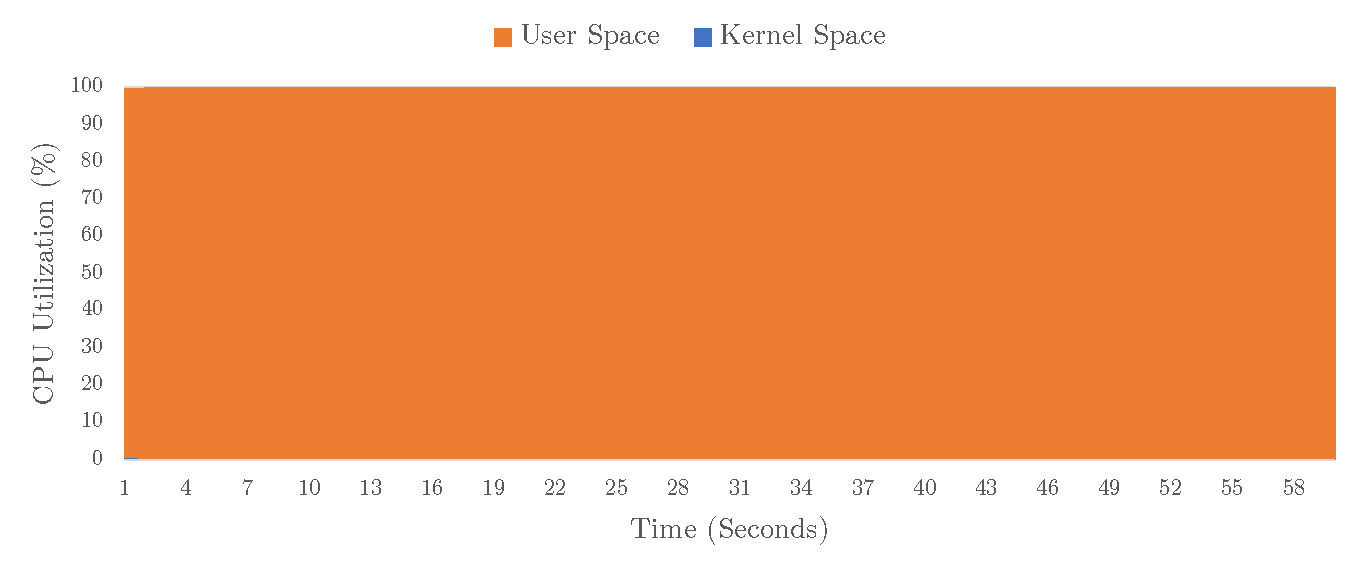
\includegraphics[width=1\linewidth]{figures/method/stress1.pdf}
    \caption{CPU Utilization during Execution of 16 stress-ng 'cpu' stressors on HPC1.}
    \label{fig:stressCPU}
\end{figure}

Figure \ref{fig:stressCPU} displays the 1-minute execution of 16 'cpu' stressors on the HPC1 system, which has 16 logical CPU cores. It is evident that the 'cpu' stressor fully utilizes this system. The load is generated in user space.

\paragraph{Generation of CPU Load in Kernel Space}
The 'get' stressor is used to generate CPU load in kernel space. This calls various system calls, which leads to a predominant CPU load in kernel space. System calls such as \texttt{getpid} (retrieving the PID of the process \cite{stress06}), \texttt{getuid} (retrieving the user ID of the process \cite{stress07}) or \texttt{gettimeofday} (retrieving the current time \cite{stress08}) are used.

\begin{figure}[h!]
    \centering
    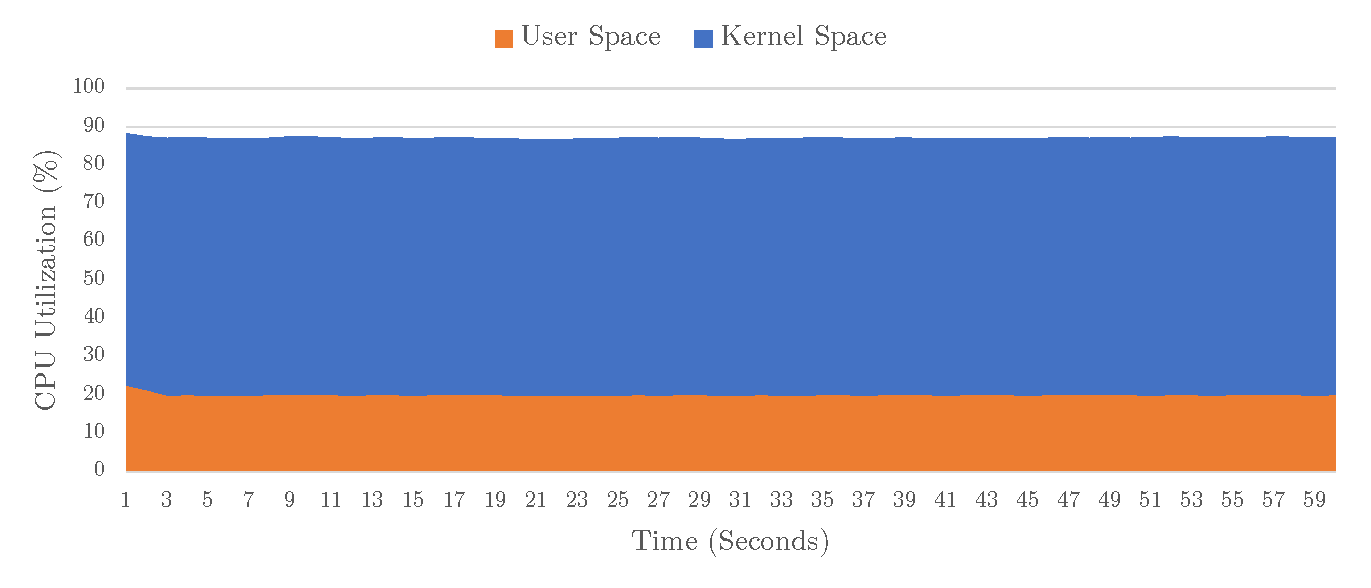
\includegraphics[width=1\linewidth]{figures/method/stress2.pdf}
    \caption{CPU Utilization during Execution of 16 stress-ng 'get' stressors on HPC1.}
    \label{fig:stressGET}
\end{figure}

Figure \ref{fig:stressGET} displays the 1-minute execution of 16 'get' stressors on the HPC1 system. The stressor utilizes approximately 87.5\% of the total system load, with 20.1\% generated in user space and 67.4\% generated in kernel space.

As can be derived from Figure \ref{fig:stressGET}, this stressor does not fully utilize a CPU core. However, it still generates 60\% to 70\% of load in kernel space on a CPU core, making it suitable for generating CPU load in kernel space during tests.

\paragraph{Generation of CPU Load by Real-Time Processes}

stress-ng allows for the specification of a scheduling policy and priority as additional options. This allows each stressor to be executed as a real-time process. For generating load, the CPU stressor described in section \ref{chap:CPUStressor} was used with the \texttt{SCHED\_FIFO} scheduling policy described in section \ref{chap:RTProcess} and a scheduling priority of 50. The scheduling priority was intentionally set lower than that of the TestSuite because communication processes have a higher priority in the distributed test system.

\subsubsection{Memory Load}
To generate memory load, the stress-ng 'bigheap' stressor is utilized. The stressor grows its heap by reallocating memory. If the Out Of Memory (OOM) killer on Linux, which is a process emplyed by the kernel when low memory is available on the system and kills one or more processes to resolve the situation \cite{stress09}, kills the process or the allocation fails then the stressor starts again.

\begin{figure}[h!]
    \centering
    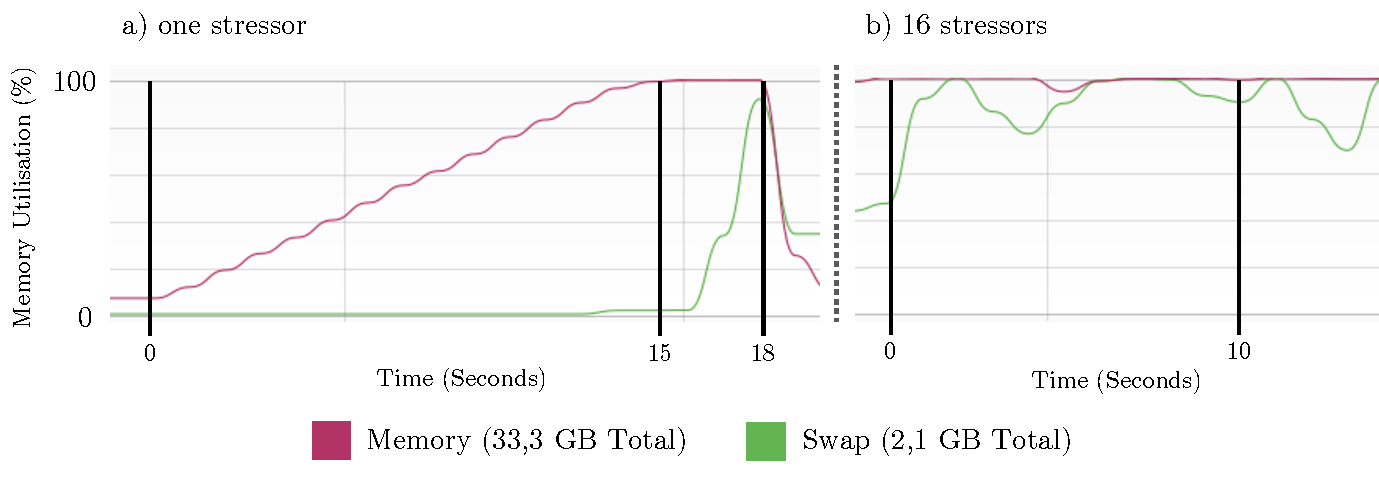
\includegraphics[width=1\linewidth]{figures/method/stress3.pdf}
    \caption{Memory Utilization during Execution of stress-ng 'bigheap' stressors on HPC1.}
    \label{fig:stressMEM}
\end{figure}

Figure \ref{fig:stressMEM} displays the memory utilization over time for a 'bigheap' stressor on HPC1 and compares it with the execution of 16 'bigheap' stressors that utilize all cores of the investigated computer system. The procedure for memory utilization is shown. The stressor requests more memory between 0 and 15 seconds until the memory is full, after which the system's swap increases. If the system has no more memory, the OOM killer terminates the process. The stressor is then restarted. If 16 'bigheap' stressors are executed simultaneously, this procedure overlaps.

The memory stressor, like any other process, also utilizes the system's CPU. Executing a memory stressor results in 100\% CPU utilization for one core.

\subsubsection{I/O Load}
The 'hdd' stressor is used to generate I/O load. It performs continuous writes to the system's hard disk.

\begin{figure}[h!]
    \centering
    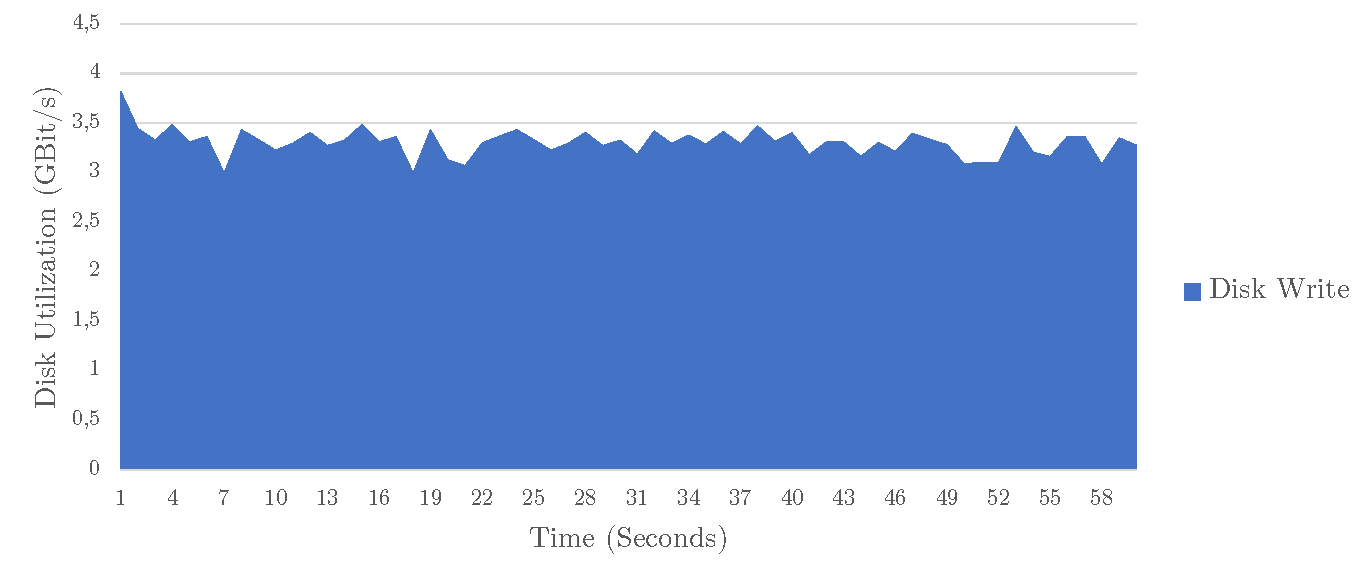
\includegraphics[width=1\linewidth]{figures/method/stress4.pdf}
    \caption{Disk Utilization during Execution of one stress-ng 'hdd' stressors on HPC1.}
    \label{fig:stressIO}
\end{figure}

Figure \ref{fig:stressIO} shows the hard disk load for a 1-minute execution of an hdd stressor. It can be seen that this performs write operations at an average data rate of around 3.2 GBit/s. Furthermore, the data rate can fluctuate between 3 GBit/s and 3.8 GBit/s. The reasons for this is that the stressor works internally with different methods and iterates through them. The methods differ, for example, in the size of the files that are written to the hard disk. The execution of an hdd stressor leads to 100\% CPU utilization of a CPU core.

Linux has I/O scheduling, which reorders and groups requests based on the logical address of the data, with the goal of improving I/O throughput \cite{stress10}. To maximize I/O device stress, I/O scheduling was disabled by selecting the "none" scheduling policy.

stress-ng does not provide a default way to limit I/O stress by limiting the data rate. To achieve this limit, Control Groups (cgroup) were used. Control groups are a kernel function that can limit the resource utilization of processes. In some tests in this work, control groups were used to limit the maximum data rate of the HDD stressor. Further information on the used cgroup2 can be found in its documentation \cite{stress11}.

\subsubsection{Interrupt Load}
The 'timer' stressor was utilized to generate load in the domain of interrupts. This produces timer events at a rate of 1 MHz, resulting in timer clock interrupts. Each timer event is then intercepted by a signal handler. The purpose of this stressor is to test the system under high interrupt load \cite{stress02}. The execution of one timer stressor also fully utilizes a CPU core to 100\%. Additionally, the system is loaded by the processing of the signal handler. The entire system's utilization was examined using an HPC as an example, which amounts to approximately 6.3\%.

It is important to note that the timer results generated in this manner differ from interrupts generated by external hardware. Although both events are asynchronous \cite{like02}, there is a significant difference between them. Timer events are generated periodically by the operating system, while hardware interrupts are triggered unpredictably by external devices such as network devices \cite{stress14}. Signal handlers execute timer events in the context of the respective process, while interrupt handlers process hardware interrupts directly in the kernel \cite{like02}.




\subsection{iPerf2}
iPerf2 is a tool for measuring bandwidth between two hosts on IP networks. It works according to the client-server principle, where the client is the sender and the server is the receiver. iPerf supports protocols such as TCP and UDP.

Various parameters can be specified when performing a measurement. These include the test duration, the datagram size or a target bandwidth. At the end of each measurement, iPerf reports the achieved bandwidth, jitter and packet losses. More information about iPerf can be found in its documentation \cite{testsuite01}.

In this work, iPerf is used with the UDP protocol for a given target and datagram size. The only goal is to generate network traffic. To measure reliability and performance characteristics, only the TestSuite presented in Section 3.3 is used as part of the thesis.